% Options for packages loaded elsewhere
\PassOptionsToPackage{unicode}{hyperref}
\PassOptionsToPackage{hyphens}{url}
\PassOptionsToPackage{dvipsnames,svgnames,x11names}{xcolor}
%
\documentclass[
  letterpaper,
  DIV=11,
  numbers=noendperiod]{scrartcl}

\usepackage{amsmath,amssymb}
\usepackage{lmodern}
\usepackage{iftex}
\ifPDFTeX
  \usepackage[T1]{fontenc}
  \usepackage[utf8]{inputenc}
  \usepackage{textcomp} % provide euro and other symbols
\else % if luatex or xetex
  \usepackage{unicode-math}
  \defaultfontfeatures{Scale=MatchLowercase}
  \defaultfontfeatures[\rmfamily]{Ligatures=TeX,Scale=1}
\fi
% Use upquote if available, for straight quotes in verbatim environments
\IfFileExists{upquote.sty}{\usepackage{upquote}}{}
\IfFileExists{microtype.sty}{% use microtype if available
  \usepackage[]{microtype}
  \UseMicrotypeSet[protrusion]{basicmath} % disable protrusion for tt fonts
}{}
\makeatletter
\@ifundefined{KOMAClassName}{% if non-KOMA class
  \IfFileExists{parskip.sty}{%
    \usepackage{parskip}
  }{% else
    \setlength{\parindent}{0pt}
    \setlength{\parskip}{6pt plus 2pt minus 1pt}}
}{% if KOMA class
  \KOMAoptions{parskip=half}}
\makeatother
\usepackage{xcolor}
\setlength{\emergencystretch}{3em} % prevent overfull lines
\setcounter{secnumdepth}{-\maxdimen} % remove section numbering
% Make \paragraph and \subparagraph free-standing
\ifx\paragraph\undefined\else
  \let\oldparagraph\paragraph
  \renewcommand{\paragraph}[1]{\oldparagraph{#1}\mbox{}}
\fi
\ifx\subparagraph\undefined\else
  \let\oldsubparagraph\subparagraph
  \renewcommand{\subparagraph}[1]{\oldsubparagraph{#1}\mbox{}}
\fi


\providecommand{\tightlist}{%
  \setlength{\itemsep}{0pt}\setlength{\parskip}{0pt}}\usepackage{longtable,booktabs,array}
\usepackage{calc} % for calculating minipage widths
% Correct order of tables after \paragraph or \subparagraph
\usepackage{etoolbox}
\makeatletter
\patchcmd\longtable{\par}{\if@noskipsec\mbox{}\fi\par}{}{}
\makeatother
% Allow footnotes in longtable head/foot
\IfFileExists{footnotehyper.sty}{\usepackage{footnotehyper}}{\usepackage{footnote}}
\makesavenoteenv{longtable}
\usepackage{graphicx}
\makeatletter
\def\maxwidth{\ifdim\Gin@nat@width>\linewidth\linewidth\else\Gin@nat@width\fi}
\def\maxheight{\ifdim\Gin@nat@height>\textheight\textheight\else\Gin@nat@height\fi}
\makeatother
% Scale images if necessary, so that they will not overflow the page
% margins by default, and it is still possible to overwrite the defaults
% using explicit options in \includegraphics[width, height, ...]{}
\setkeys{Gin}{width=\maxwidth,height=\maxheight,keepaspectratio}
% Set default figure placement to htbp
\makeatletter
\def\fps@figure{htbp}
\makeatother
\newlength{\cslhangindent}
\setlength{\cslhangindent}{1.5em}
\newlength{\csllabelwidth}
\setlength{\csllabelwidth}{3em}
\newlength{\cslentryspacingunit} % times entry-spacing
\setlength{\cslentryspacingunit}{\parskip}
\newenvironment{CSLReferences}[2] % #1 hanging-ident, #2 entry spacing
 {% don't indent paragraphs
  \setlength{\parindent}{0pt}
  % turn on hanging indent if param 1 is 1
  \ifodd #1
  \let\oldpar\par
  \def\par{\hangindent=\cslhangindent\oldpar}
  \fi
  % set entry spacing
  \setlength{\parskip}{#2\cslentryspacingunit}
 }%
 {}
\usepackage{calc}
\newcommand{\CSLBlock}[1]{#1\hfill\break}
\newcommand{\CSLLeftMargin}[1]{\parbox[t]{\csllabelwidth}{#1}}
\newcommand{\CSLRightInline}[1]{\parbox[t]{\linewidth - \csllabelwidth}{#1}\break}
\newcommand{\CSLIndent}[1]{\hspace{\cslhangindent}#1}

\usepackage{booktabs}
\usepackage{longtable}
\usepackage{array}
\usepackage{multirow}
\usepackage{wrapfig}
\usepackage{float}
\usepackage{colortbl}
\usepackage{pdflscape}
\usepackage{tabu}
\usepackage{threeparttable}
\usepackage{threeparttablex}
\usepackage[normalem]{ulem}
\usepackage{makecell}
\usepackage{xcolor}
\KOMAoption{captions}{tableheading}
\usepackage[left]{lineno}
\linenumbers
\makeatletter
\makeatother
\makeatletter
\makeatother
\makeatletter
\@ifpackageloaded{caption}{}{\usepackage{caption}}
\AtBeginDocument{%
\ifdefined\contentsname
  \renewcommand*\contentsname{Table of contents}
\else
  \newcommand\contentsname{Table of contents}
\fi
\ifdefined\listfigurename
  \renewcommand*\listfigurename{List of Figures}
\else
  \newcommand\listfigurename{List of Figures}
\fi
\ifdefined\listtablename
  \renewcommand*\listtablename{List of Tables}
\else
  \newcommand\listtablename{List of Tables}
\fi
\ifdefined\figurename
  \renewcommand*\figurename{Figure}
\else
  \newcommand\figurename{Figure}
\fi
\ifdefined\tablename
  \renewcommand*\tablename{Table}
\else
  \newcommand\tablename{Table}
\fi
}
\@ifpackageloaded{float}{}{\usepackage{float}}
\floatstyle{ruled}
\@ifundefined{c@chapter}{\newfloat{codelisting}{h}{lop}}{\newfloat{codelisting}{h}{lop}[chapter]}
\floatname{codelisting}{Listing}
\newcommand*\listoflistings{\listof{codelisting}{List of Listings}}
\makeatother
\makeatletter
\@ifpackageloaded{caption}{}{\usepackage{caption}}
\@ifpackageloaded{subcaption}{}{\usepackage{subcaption}}
\makeatother
\makeatletter
\@ifpackageloaded{tcolorbox}{}{\usepackage[many]{tcolorbox}}
\makeatother
\makeatletter
\@ifundefined{shadecolor}{\definecolor{shadecolor}{rgb}{.97, .97, .97}}
\makeatother
\makeatletter
\makeatother
\ifLuaTeX
  \usepackage{selnolig}  % disable illegal ligatures
\fi
\IfFileExists{bookmark.sty}{\usepackage{bookmark}}{\usepackage{hyperref}}
\IfFileExists{xurl.sty}{\usepackage{xurl}}{} % add URL line breaks if available
\urlstyle{same} % disable monospaced font for URLs
\hypersetup{
  pdftitle={Values disclosures and trust in science: A replication study},
  colorlinks=true,
  linkcolor={blue},
  filecolor={Maroon},
  citecolor={Blue},
  urlcolor={Blue},
  pdfcreator={LaTeX via pandoc}}

\title{Values disclosures and trust in science: A replication study}
\author{}
\date{}

\begin{document}
\maketitle
\begin{abstract}
While philosophers of science generally agree that social, political,
and ethical values can play legitimate roles in science, there is active
debate over whether scientists should disclosure such values in their
public communications. This debate depends, in part, on empirical claims
about whether values disclosures might undermine public trust in
science. In a previous study, Elliott et al.~used an online experiment
to test this empirical claim. The current paper reports a replication
attempt of their experiment. Comparing results of the original study and
our replication, we do not find evidence for a transparency penalty or
``shared values'' effect, but do find evidence that the content of
scientific conclusions (whether or not a chemical is found to cause
harm) might effect perceived trustworthiness and that scientists who
value public health and disclose this value might be perceived as more
trustworthy.
\end{abstract}
\ifdefined\Shaded\renewenvironment{Shaded}{\begin{tcolorbox}[sharp corners, enhanced, frame hidden, breakable, borderline west={3pt}{0pt}{shadecolor}, boxrule=0pt, interior hidden]}{\end{tcolorbox}}\fi

Daniel J. Hicks\textsuperscript{1*}, Emilio Lobato\textsuperscript{1}\\
\textsuperscript{1}: University of California, Merced, 5200 N Lake Road,
Merced, CA, 95343\\
\textsuperscript{*}: Address correspondence to
\href{mailto:dhicks4@ucmerced.edu}{\nolinkurl{dhicks4@ucmerced.edu}}\\
\strut \\
Keywords: trust, trust in science, values in science, replication,
philosophy of science

\hypertarget{introduction}{%
\section{Introduction}\label{introduction}}

Over the past 15 years, many philosophers of science have rejected the
ideal of value-free science and related, traditional understandings of
objectivity and political neutrality of science (Douglas 2009; Elliott
2017). According to the value-free ideal, social and political values
--- such as feminism, environmentalism, or the protection of human
health --- have no legitimate role to play in the evaluation of
scientific hypotheses. The value-free ideal is compatible with allowing
social and political values to play important roles earlier and later in
inquiry. Specifically, these values may legitimately shape the content
and framing of research questions --- researchers might decide to
investigate whether chemical X causes cancer out of a concern to protect
human health --- and will be essential when scientific findings are used
to inform public policy --- say, banning the use of chemical X. But,
according to the value-free ideal, these values must not influence the
collection and analysis of data and the process of reaching an overall
conclusion about whether or not chemical X causes cancer.

Challenges to the value-free ideal argue that at least some social and
political values may, or even should, play a role in the evaluation of
scientific hypotheses. Keeping with the example, the question of whether
chemical X causes cancer has much more significant social and political
implications than the question of whether chemical X fluoresces under
ultraviolet light. So, in the interest of protecting human health, it
would be appropriate to \emph{scientifically} accept the hypothesis that
chemical X is carcinogenic for regulatory purposes based on relatively
weak or provisional evidence (Cranor 1995; Elliott and McKaughan 2014;
Fernández Pinto and Hicks 2019).

While this kind of argument indicates that at least some social and
political values may or should play at least some role in the evaluation
of at least some scientific hypotheses, it doesn't provide us with much
positive guidance: which values, playing which roles, in the evaluation
of which hypotheses? (Hicks 2014) One (partial) answer to this set of
questions appeals to the ideal of transparency: scientists should
disclose to the public the social and political values that have
influenced their research (Elliott and Resnik 2014; McKaughan and
Elliott 2013). But some philosophers have objected to this transparency
proposal, arguing that it might undermine trust in science.

Specifically, ethicists make a distinction between trust and
trustworthiness (Baier 1986). Trust is a verb: placing one's trust in
someone else, with respect to some activity or domain. Trustworthiness
is an assessment, of whether or not that trust is appropriate. According
to the objection to the ideal of transparency, transparency would not
change how trustworthy science actually is --- the science is conducted
in the same way --- but might reduce public perceptions of
trustworthiness --- as members of the public see how the scientific
sausage is made. For instance, members of the public generally accept
the ideal of value-free science; values disclosures would violate this
ideal, making scientists (incorrectly) appear biased and untrustworthy
(John 2017; Kovaka 2021).

This objection is an empirical prediction: if scientists disclose their
values, they will be perceived as less trustworthy. Elliott et al.
(2017) conducted an online survey study to evaluate this prediction. The
authors found tentative evidence that disclosing values may reduce the
perceived trustworthiness of a scientist, and that this effect may be
moderated by whether or not participants share the same values as the
scientist and whether or not the scientist reports findings contrary to
their stated values. However, these authors collected data from a
somewhat small sample using Amazon Mechanical Turk, and adopted an
analytical approach that diluted their sample across different
conditions. In this paper, we report the results of a replication of
Elliott et al. (2017) study 1, using a larger sample and a more
statistically efficient analytical approach. The major results found by
Elliott et al. (2017) serve as the basis for our hypotheses, described
below.

\hypertarget{methods-and-materials}{%
\section{Methods and Materials}\label{methods-and-materials}}

\hypertarget{experimental-design}{%
\subsection{Experimental design}\label{experimental-design}}

We used the same experimental stimulus and design as Elliott et al.
(2017), which we embedded within a larger project examining the public's
perceptions of the values in science. In this paper, we are only
reporting the replication component of the project. The replication
component was the same 3 (Values: No Disclosure, Economic Growth, Public
Health) \times 2 (Harm: Causes Harm, Does Not Cause Harm) experimental
design as used by Elliott et al. (2017). In each condition, participants
are first shown a single presentation slide and the following
explanatory text:

\begin{quote}
For several decades, a scientist named Dr.~Riley Spence has been doing
research on chemicals used in consumer products. One
chemical---Bisphenol A, popularly known as BPA---is found in a large
number of consumer products and is suspected of posing risks to human
health. Yet, scientists do not agree about these possible health risks.
Dr.~Spence recently gave a public talk in Washington, D.C., about BPA
research. Here is the final slide from Dr.~Spence's presentation.
\end{quote}

No other information about the (fictional) Dr.~Spence is provided. The
content of the slide varies across the conditions
(Figure~\ref{fig-stimulus}). Each slide has the header ``My
conclusion,'' followed by a list of 2 or 3 bullets. The first bullet, if
present, makes a values disclosure, stating that either economic growth
or public health should be a top national priority. This first bullet is
not present in the ``no disclosure'' values condition. The second
bullet, identical across conditions, states ``I examined the scientific
evidence on potential health risks of BPA.'' The third bullet concludes
that BPA either does or does not cause harm to people, depending on
whether the subject is in the ``causes harm'' or ``does not cause harm''
condition.

\begin{figure}

{\centering 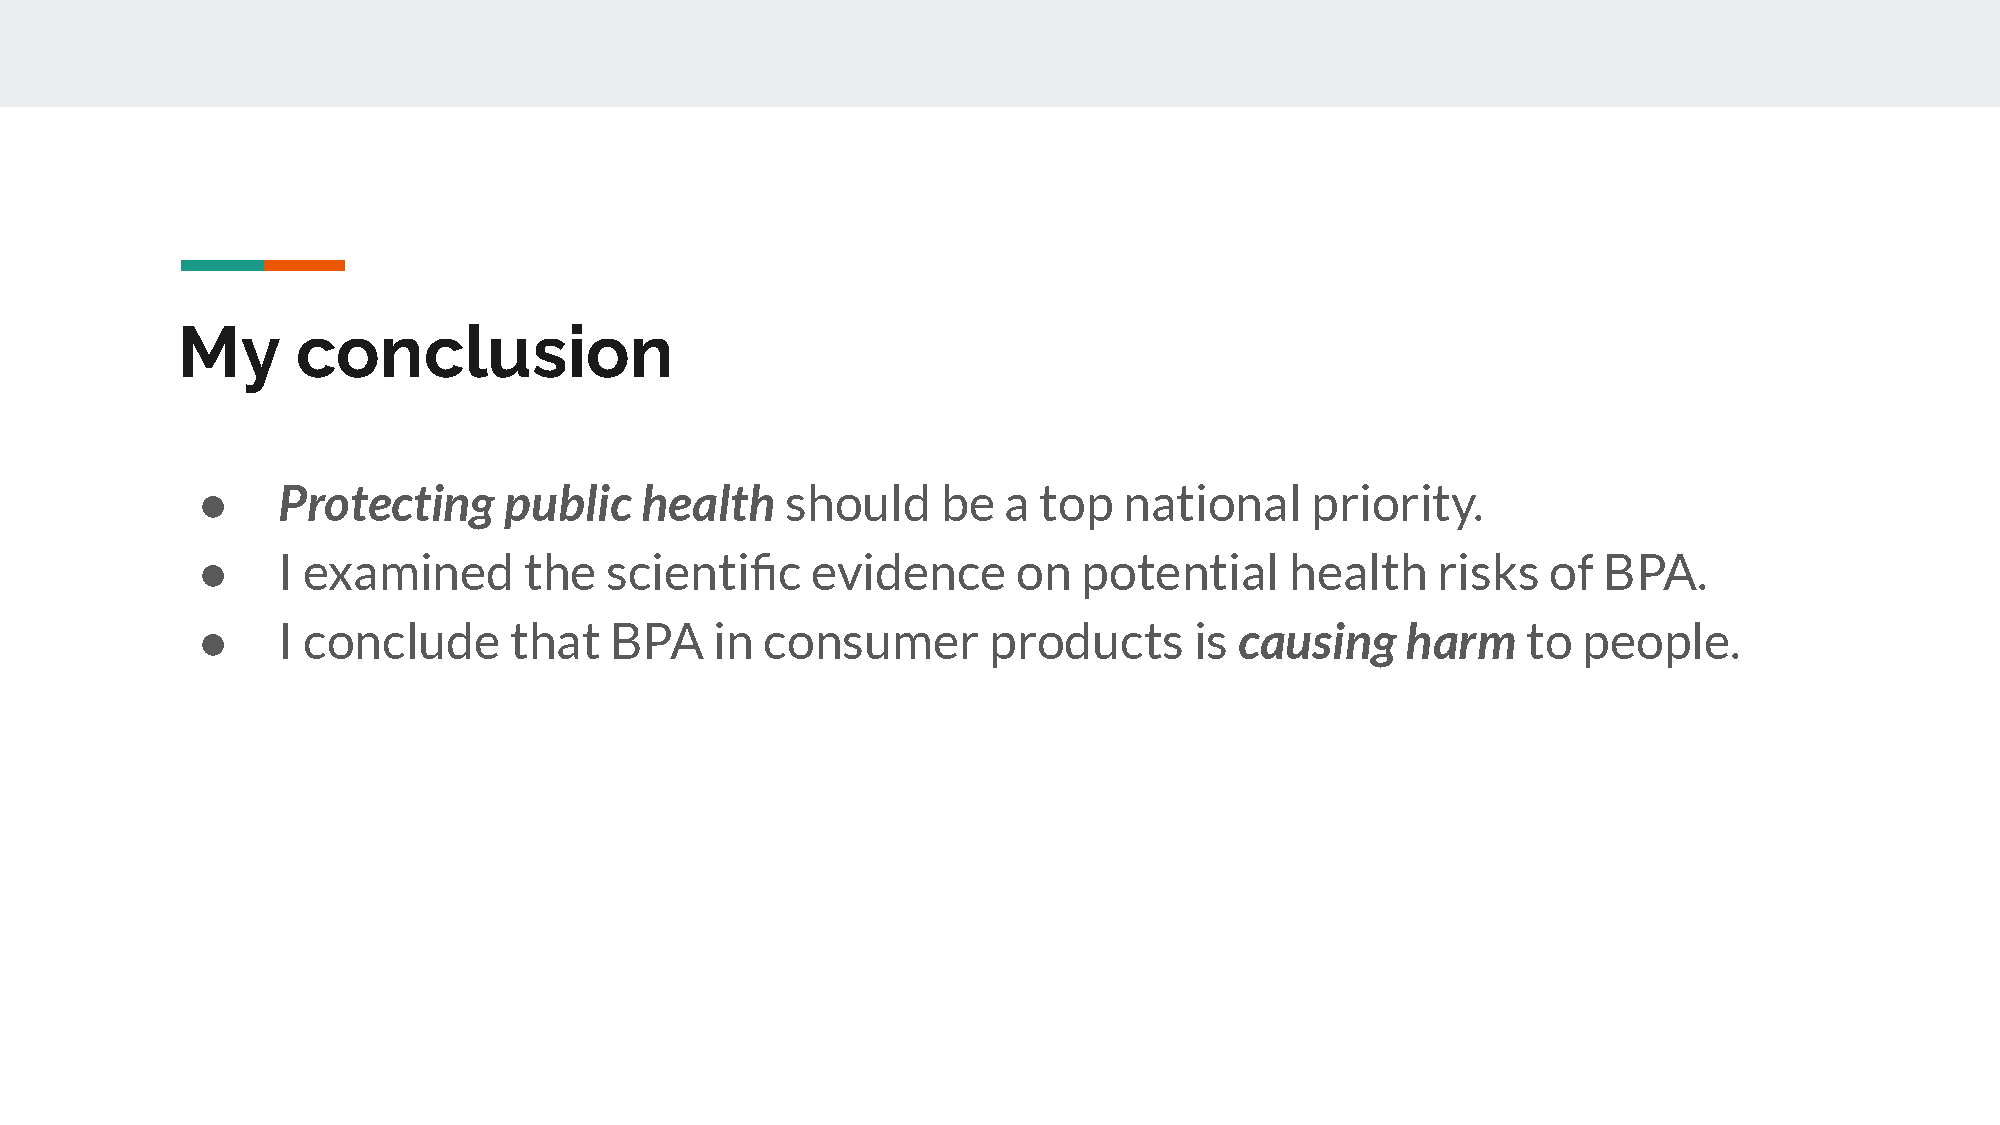
\includegraphics{fig1_stimulus.png}

}

\caption{\label{fig-stimulus}Example of the experimental stimulus, from
the ``public health values disclosure'' + ``causes harm'' conclusion.}

\end{figure}

After viewing the slide, the participant is then asked to rate
Dr.~Spence's trustworthiness using a semantic differential scale.
Elliott et al. (2017) used an ad hoc scale; we used the Muenster
Epistemic Trustworthiness Inventory (METI; Hendriks, Kienhues, and
Bromme 2015), which substantially overlaps but is not identical to the
Elliott et al. (2017) scale. Even though the ad hoc scale created by
Elliot and colleagues had acceptable internal reliability, the METI was
developed and psychometrically validated to measure the perceived
trustworthiness of experts. On the METI, participants rate the target
scientist (the fictional Dr.~Spence) on a 1-7 scale for 14 semantic
differential items, where each item is anchored at the ends by a pair of
words, such as competent-incompetent or responsible-irresponsible. The
METI scale captures perceived trustworthiness of a target along three
dimensions: competence, benevolence, and integrity. However, the three
dimensions were strongly correlated in our sample (Pearson r values
ranging from .75 to .92). To avoid issues of multicollinearity in our
analyses, we averaged participant scores into a single composite
measure. In both Elliott et al. (2017) and our replication analysis, all
items were averaged together to form a 1-7 composite measure of
trustworthiness. To aid interpretation, in the analysis the direction of
the scale has been set so that increased values correspond to increased
perceived trustworthiness.

As its name indicates, METI assesses perceived trustworthiness rather
than trust (such as accepting Dr.~Spence's conclusion about BPA). It is
conceivable that participants might trust Dr.~Spence's conclusion even
if they judge Spence to be untrustworthy, or vice versa. But we would
typically trust and trustworthiness to go together.

Elliott et al. (2017) explain that they selected BPA as a complex,
ongoing, public scientific controversy. For our replication, we chose to
keep BPA, rather than switching to a different public scientific
controversy with a higher profile in 2021, such as climate change,
police violence, voter fraud, or any of numerous aspects of the COVID-19
pandemic. All of these controversies are highly politically charged,
with prominent public experts and counterexperts (Goldenberg 2021,
100--101, ch.~6). While we anticipated some effects of political
partisanship in the BPA case, we felt it would be less likely to swamp
the values disclosure that was our primary interest.

After filling in the METI, participants provided demographic
information, including self-identifying their political ideology, and
other sections of the survey that are not examined here. Due to
researcher error, a question about the participants' values (whether
they prioritize economic growth or public health) was omitted in the
first wave of data collection; this question was asked in a followup
wave.

\hypertarget{replication-hypotheses-and-analytical-approach}{%
\subsection{Replication hypotheses and analytical
approach}\label{replication-hypotheses-and-analytical-approach}}

We identified 5 major findings from Elliott et al. (2017) for our
replication attempt:

\begin{description}
\tightlist
\item[H1. Modest correlation between values and ideology]
(a) Political liberals are more likely to prioritize public health over
economic growth, compared to political conservatives; but (b) a majority
of political conservatives prioritize public health.
\item[H2. Consumer risk sensitivity]
Scientists who find that a chemical harms human health are perceived as
more trustworthy than scientists who find that a chemical does not cause
harm.
\item[H3. Transparency penalty]
Scientists who disclose values are perceived as less trustworthy than
scientists who do not.
\item[H4. Shared values]
Given that the scientist discloses values, if the participant and the
scientist share the same values, the scientist is perceived as more
trustworthy than if the participant and scientist have discordant
values.
\item[H5. Variation in effects]
The magnitude of the effects for hypotheses 2-4 vary depending on
whether the participant prioritizes public health or economic growth.
\end{description}

Hypothesis H3, the transparency penalty, corresponds to the objection to
transparency: disclosing values undermines trust in science. However,
the shared values effect works in the opposite direction, counteracting
the transparency penalty.

Hypothesis 1 was analyzed using Spearman rank order correlation to test
H1a and a visual inspection of descriptive statistics to test H1b.
Hypotheses 2-5 were analyzed using linear regression models as a common
framework, with a direct acyclic graph (DAG) constructed \emph{a priori}
to identify appropriate adjustments (covariates) for H4 and 5. Because
Elliott et al. (2017) made their data publicly available, and our
analytical approaches differ somewhat from theirs, we conducted parallel
analyses of their data, and report these parallel results for H2 and 3.
Exploratory data analysis was used throughout to support data validation
and aid interpretation.

\hypertarget{participants}{%
\subsection{Participants}\label{participants}}

Participants were recruited using the online survey platform Prolific,
and the survey was administered in a web browser using Qualtrics.
Prolific has an option to draw samples that are balanced to be
representative by age, binary gender, and a 5-category race variable
(taking values Asian, Black, Mixed, Other, and White) for US adults
({``Representative Samples FAQ''} 2022). A recent analysis finds that
Prolific produces substantially higher quality data than Amazon
Mechanical Turk for online survey studies, though three of the five
authors are affiliated with Prolific (Peer et al. 2021). Preliminary
power analysis recommended a sample of approximately 1,000 participants
to reliably detect non-interaction effects (H1-4).

After excluding participants who declined consent after opening the
survey or did not complete the survey, we had 988 participants in the
full analysis sample (\(M_{age}\) = 44-years-old, \(SD_{age}\) =
16-years, Woman/Female = 498, Man/Male = 458, White = 712, Black = 124,
Asian or Pacific Islander = 63, Hispanic = 33, American Indian or
Alaskan Native = 5, Mixed or Other = 51). Participants were randomly
assigned to condition, with 163 assigned to the No Disclosure + Causes
Harm condition, 165 assigned to the No Disclosure + Does Not Cause Harm
condition, 165 assigned to the Economic Growth + Causes Harm condition,
165 assigned to the Economic Growth + Does Not Cause Harm condition, 168
assigned to the Public Health + Causes Harm condition, and 162 assigned
to the Public Health + Does Not Cause Harm condition
(Table~\ref{tbl-condition}). Due to researcher error a question about
participants' values was not included in the original survey. Of the
full 988 participants, 844 participants (85\%) responded to the followup
question about their own values (participant prioritizes economic growth
or public health). Consequently, subsamples for hypotheses 4 and 5 were
substantially smaller than the full analysis sample.

\hypertarget{tbl-condition}{}
\begin{table}
\caption{\label{tbl-condition}Assignment of participants to conditions }\tabularnewline

\centering
\resizebox{\linewidth}{!}{
\begin{tabular}{lcc}
\toprule
\textbf{Characteristic} & \textbf{causes harm}, N = 496 & \textbf{does not cause harm}, N = 492\\
\midrule
disclosure/values &  & \\
\hspace{1em}no disclosure & 163 (33\%) & 165 (34\%)\\
\hspace{1em}public health & 168 (34\%) & 162 (33\%)\\
\hspace{1em}economic growth & 165 (33\%) & 165 (34\%)\\
\bottomrule
\multicolumn{3}{l}{\rule{0pt}{1em}\textsuperscript{1} n (\%)}\\
\end{tabular}}
\end{table}

The study was approved by the UC Merced IRB on August 17, 2021, and data
collection ran October 18-20, 2021. The followup survey asking the
initial sample of participants about their own values regarding economic
growth and public health was conducted December 8, 2021 through March 5,
2022.

\hypertarget{software-and-reproducibility}{%
\subsection{Software and
reproducibility}\label{software-and-reproducibility}}

Data cleaning and analysis was conducted in R version 4.1.2 (R Core Team
2021), with extensive use of the \texttt{tidyverse} suite of packages
version 1.3.1 (Wickham et al. 2019). Regression tables were generated
using the packages \texttt{gt} version 0.5.0 (Iannone, Cheng, and
Schloerke 2022) and \texttt{gtsummary} version 1.6.0 (Sjoberg et al.
2021).

Anonymized original data and reproducible code are available at
\url{https://github.com/dhicks/transparency}. Instructions in that
repository explain how to automatically reproduce our analysis.

\hypertarget{results}{%
\section{Results}\label{results}}

Critically, our data are unlikely to be representative by education
level and political ideology. In 2021, about 9\% of US adults 25 or over
had a less than high school education, and 38\% had a Bachelor's degree
or higher ({``CPS Historical Time Series Visualizations''} 2022, fig.
2). Only 1\% of our participants reported a less than high school
education, and 57\% reported a Bachelor's degree or higher. For
political ideology, the General Social Survey has consistently found
over several decades that about 30\% of US adults identify as liberal,
about 30\% identify as conservative, and about 40\% as moderate ({``GSS
Data Explorer''} 2022). Among our participants, liberals (574) heavily
outnumber conservatives (248; Figure~\ref{fig-part-values}). Both
overrepresentation of college graduates and underrepresentation of
conservatives (especially conservatives with strong anti-institutional
views) are known issues in public opinion polling (Kennedy et al. 2018).
In exploratory data analysis, we noted that there was essentially no
correlation between political ideology and perceived trustworthiness (in
the online supplement, see subsection H5-shared). This was surprising,
since general trust/distrust in science has become a partisan phenomenon
over the last few decades: data from the General Social Survey shows
increasing trust in science from liberals and decreasing trust from
conservatives (Gauchat 2012; Lee 2021), and many (though not all)
prominent public scientific controversies align with
liberal-conservative partisanship (Funk and Rainie 2015).

Because of these representation issues, insofar as some political
conservatives are both less likely to participate in studies on Prolific
(or at least in our particular study) and likely to perceive Spence as
less trustworthy, this will produce omitted variable bias for analyses
that require adjustment by political ideology. Analysis of our \emph{a
priori} DAG indicated that, for the hypotheses examined here, this
adjustment was not necessary in any case. When some adjustment was
necessary (H4-5), we included political ideology along with other
demographic variables in an alternative model specification as a
robustness check. In line with the DAG, in no case did these robustness
checks produce indications of omitted variable bias.

\hypertarget{h1-correlation-between-values-and-ideology}{%
\subsection{H1: Correlation between values and
ideology}\label{h1-correlation-between-values-and-ideology}}

We tested the hypothesis of a modest correlation between values and
ideology in two ways. First, to test (H1a) whether political liberals
are more likely to prioritize public health over economic growth
compared to conservatives, we conducted a Spearman's rank order
correlation. Results revealed a significant correlation in line with the
hypothesis, Spearman's \(\rho\) = -.47, \emph{p} \textless{} .001.
Political liberals were more likely than conservatives to value public
health over economic growth. To test (H1b) that a majority of political
conservatives priortize public health over economic growth we
cross-tabulated the data. Results revealed that, contrary to the
hypothesis, slightly more than half of the self-reported political
conservatives in our sample reported valuing economic growth (51.7\%)
over public health (48.3\%). See Figure~\ref{fig-part-values}.

\begin{figure}

{\centering 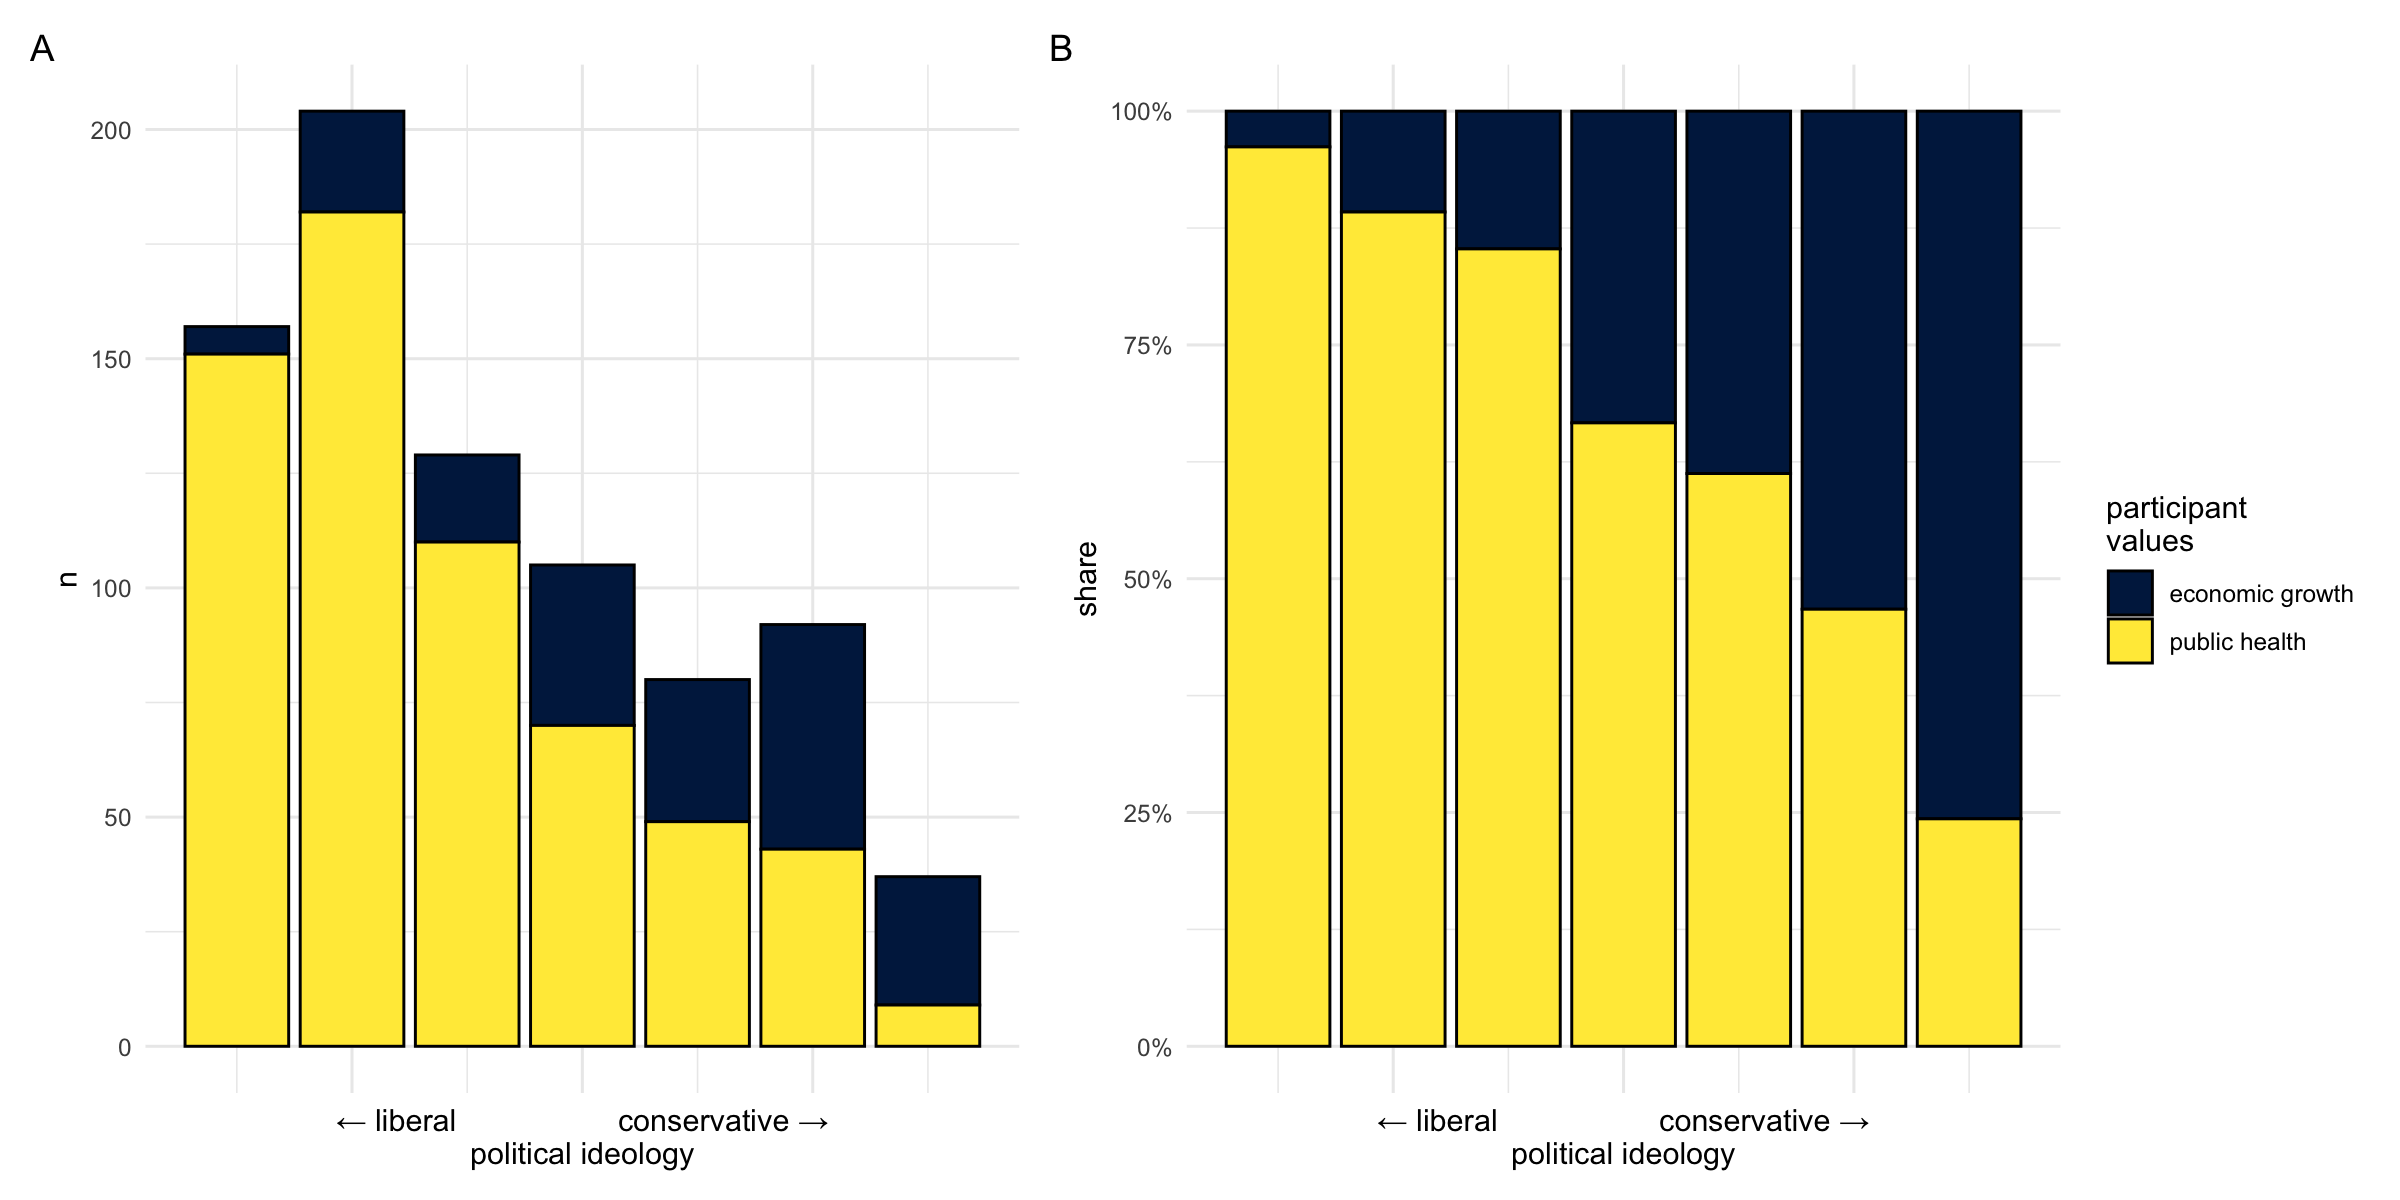
\includegraphics{fig2_part_values.png}

}

\caption{\label{fig-part-values}Participant values by political
ideology. (A) Absolute counts, (B) shares within political ideology
categories. Panel (A) shows that our sample substantially
over-represents political liberals.}

\end{figure}

\hypertarget{h2-and-h3-consumer-risk-sensitivity-and-transparency-penalty}{%
\subsection{H2 and H3: Consumer risk sensitivity and transparency
penalty}\label{h2-and-h3-consumer-risk-sensitivity-and-transparency-penalty}}

Next, we tested the hypotheses that (H2) scientists who find a chemical
harms human health are perceived as more trustworthy than scientist who
find that a chemical does not cause harm and (H3) a scientist who
discloses values are perceived as less trustworthy than a scientist who
does not. For this analysis, we regressed participants' METI ratings
onto both the Conclusions and Disclosure experimental conditions. The
full model was significant, adj. \(R^2\) = .148, \emph{F}(2, 985) =
86.59, \emph{p} \textless{} .001 (see Table~\ref{tbl-bc}). Specifically,
results revealed that the conclusions reported by the scientist
predicted participants' perceived trustworthiness in line with our
hypothesis. Participants rated the scientist who reported that BPA does
not cause harm as less trustworthy (\(M_{sd} = 4.48_{1.26}\)) than the
scientist who reported that BPA causes harm (\(M_{sd} = 5.47_{1.12}\)),
\(\beta\) = -0.99, \emph{t}(985) = -13.09, \emph{p} \textless{} .001. By
contrast, the results do not provide evidence in favor of our hypothesis
that a scientist disclosing their values (\(M_{sd} = 4.94_{1.33}\)) are
perceived as less trustworthy than a scientist who does not disclose
values (\(M_{sd} = 5.05_{1.21}\)), \(\beta\) = -0.12, \emph{t}(985) =
-1.46, \emph{p} = .143.

\hypertarget{tbl-bc}{}
\begin{table}
\caption{\label{tbl-bc}Regression analysis for hypotheses H2 (consumer risk sensitivity) and H3
(disclosure effect) }\tabularnewline

\centering
\resizebox{\linewidth}{!}{
\begin{tabular}{lcccccc}
\toprule
\multicolumn{1}{c}{ } & \multicolumn{3}{c}{\textbf{EMAD}} & \multicolumn{3}{c}{\textbf{HL replication}} \\
\cmidrule(l{3pt}r{3pt}){2-4} \cmidrule(l{3pt}r{3pt}){5-7}
\textbf{Characteristic} & \textbf{Beta} & \textbf{95\% CI} & \textbf{p-value} & \textbf{Beta} & \textbf{95\% CI} & \textbf{p-value}\\
\midrule
(Intercept) & 6.0 & 5.7, 6.2 & <0.001 & 5.6 & 5.4, 5.7 & <0.001\\
conclusion &  &  &  &  &  & \\
\hspace{1em}conclusion[does not cause harm] & -1.1 & -1.3, -0.82 & <0.001 & -1.0 & -1.1, -0.84 & <0.001\\
disclosure &  &  &  &  &  & \\
\hspace{1em}disclosure[TRUE] & -0.52 & -0.78, -0.26 & <0.001 & -0.12 & -0.28, 0.04 & 0.14\\
\midrule
\addlinespace
R² & 0.152 &  &  & 0.150 &  & \\
No. Obs. & 498 &  &  & 988 &  & \\
Adjusted R² & 0.148 &  &  & 0.148 &  & \\
Statistic & 44.3 &  &  & 86.6 &  & \\
p-value & <0.001 &  &  & <0.001 &  & \\
\bottomrule
\multicolumn{7}{l}{\rule{0pt}{1em}\textsuperscript{1} CI = Confidence Interval}\\
\end{tabular}}
\end{table}

\hypertarget{h4-shared-values}{%
\subsection{H4: Shared values}\label{h4-shared-values}}

Next, we tested the hypothesis that (H4) if the participant and
scientist share the same values, the scientist is perceived as more
trustworthy than if the participant and scientist do not share the same
values. For this and related analyses, we only included data from
participants who were assigned to either of the Disclosure conditions
and self-reported their own values, reducing the sample to 567.
Following this, we created a new Shared Values variable as a composite
of the participants' reported values and the scientist's values. For
this analysis, an a priori directed acyclic graphic (DAG) indicated that
a univariate regression of participants' METI rating onto Shared Values
would produce a biased estimate, that adjustments were required for both
the participant's and scientist's values, and that including demographic
variables would not effect this estimate (Figure~\ref{fig-shared-dag}).
While the univariate model was significant, adj. \(R^2\)= .029,
\emph{F}(1, 565) = 18.0, \emph{p} \textless{} .001
(Table~\ref{tbl-shared} model 1), after adjusting for scientist values
Shared Values did not emerge as a significant predictor of participants'
perceptions of the trustworthiness of the scientist
(Table~\ref{tbl-shared} models 2-4), indicating that the univariate
estimate was indeed biased. Rather, only the scientist's disclosed
values significantly predicted how trustworthy participants rated the
scientist, such that a scientist who disclosed valuing public health was
rated as more trustworthy than a scientist who disclosed valuing
economic growth. This scientist values effect was robust across
alternative model specifications, with an estimated effect of 0.6 (95\%
CI 0.4-0.8; Table~\ref{tbl-shared} models 2-5), again consistent with
the DAG.

\begin{figure}

{\centering 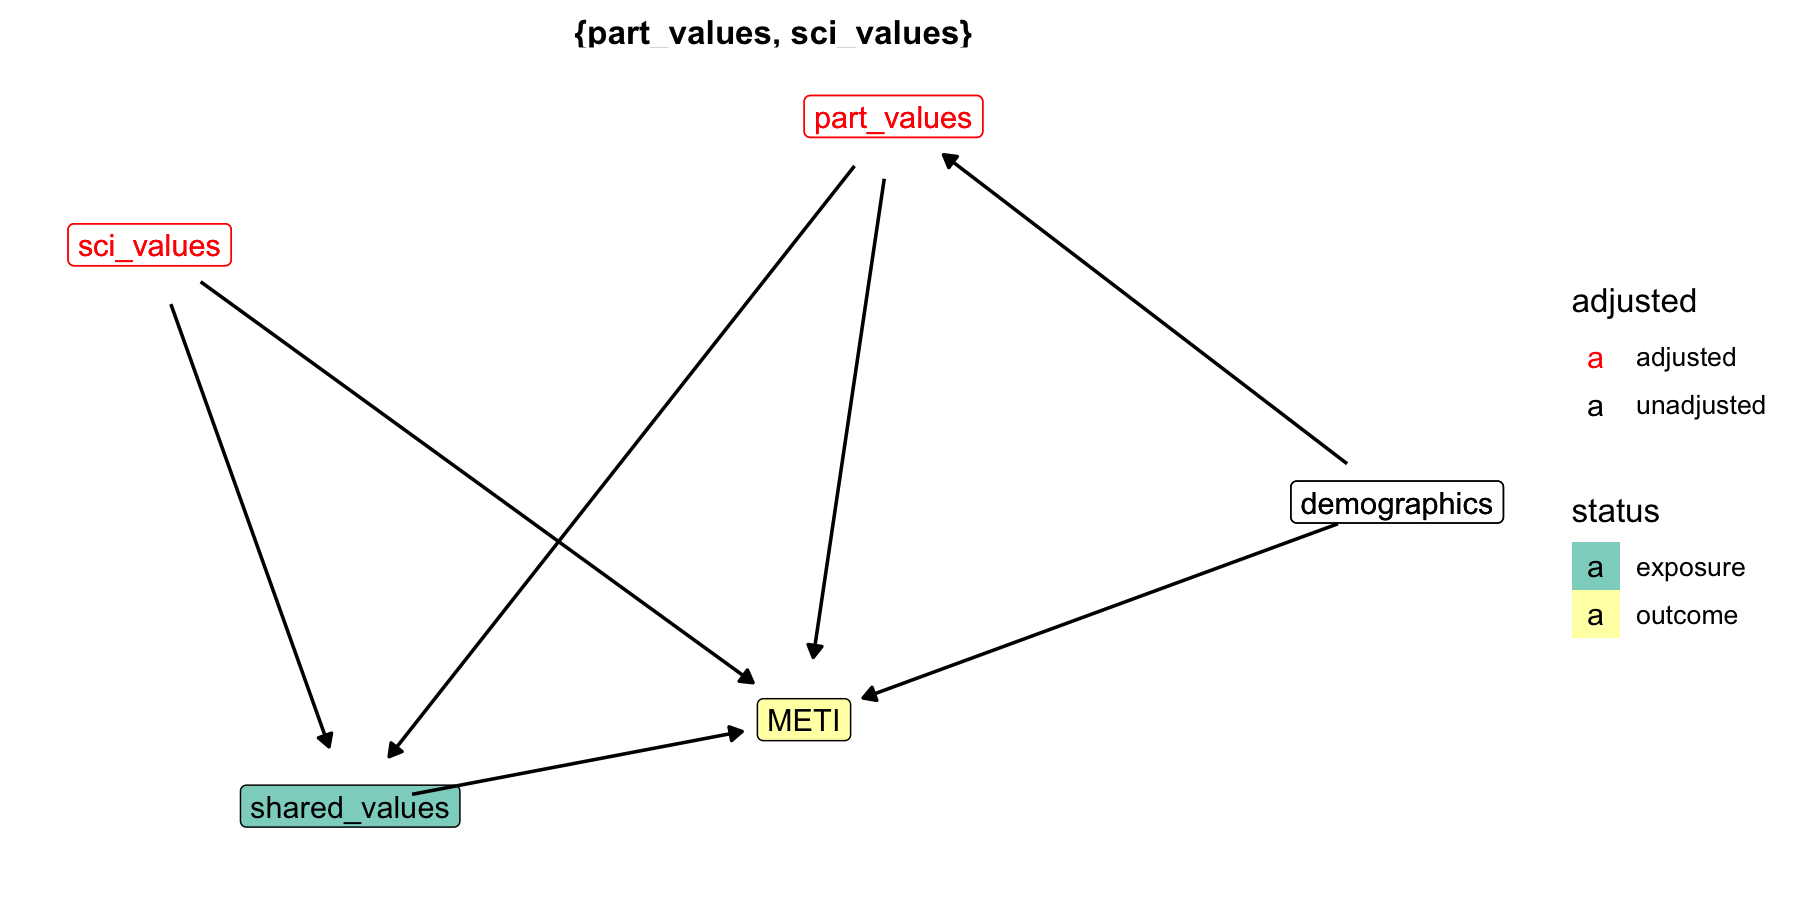
\includegraphics{fig3_shared_values_dag.png}

}

\caption{\label{fig-shared-dag}Directed acyclic graph (DAG) for analysis
of the shared values effect. If the DAG is faithful, adjusting for
scientist values (\texttt{sci\_values}) and participant values
(\texttt{part\_values}) is sufficient for estimating the effect of
shared values on perceived trustworthiness (\texttt{METI}). In
particular, adjusting for demographics should not change the regression
coefficient on shared values.}

\end{figure}

\hypertarget{tbl-shared}{}
\begin{table}
\caption{\label{tbl-shared}Sequential regression analysis of hypothesis H4 shared values/scientist
values effects }\tabularnewline

\centering
\resizebox{\linewidth}{!}{
\begin{tabular}{lccccccccccccccc}
\toprule
\multicolumn{1}{c}{ } & \multicolumn{3}{c}{(1) univariate} & \multicolumn{3}{c}{(2) scientist values} & \multicolumn{3}{c}{(3) participant values} & \multicolumn{3}{c}{(4) demographics} & \multicolumn{3}{c}{(5) scientist values alone} \\
\cmidrule(l{3pt}r{3pt}){2-4} \cmidrule(l{3pt}r{3pt}){5-7} \cmidrule(l{3pt}r{3pt}){8-10} \cmidrule(l{3pt}r{3pt}){11-13} \cmidrule(l{3pt}r{3pt}){14-16}
\textbf{Characteristic} & \textbf{Beta} & \textbf{95\% CI} & \textbf{p-value} & \textbf{Beta} & \textbf{95\% CI} & \textbf{p-value} & \textbf{Beta} & \textbf{95\% CI} & \textbf{p-value} & \textbf{Beta} & \textbf{95\% CI} & \textbf{p-value} & \textbf{Beta} & \textbf{95\% CI} & \textbf{p-value}\\
\midrule
(Intercept) & 4.7 & 4.5, 4.9 & <0.001 & 4.6 & 4.4, 4.7 & <0.001 & 4.7 & 4.5, 5.0 & <0.001 & 4.5 & 3.7, 5.3 & <0.001 & 4.6 & 4.5, 4.8 & <0.001\\
shared values &  &  &  &  &  &  &  &  &  &  &  &  &  &  & \\
\hspace{1em}shared\_values[TRUE] & 0.47 & 0.25, 0.68 & <0.001 & 0.11 & -0.15, 0.37 & 0.4 & 0.10 & -0.16, 0.36 & 0.5 & 0.07 & -0.21, 0.35 & 0.6 &  &  & \\
scientist values &  &  &  &  &  &  &  &  &  &  &  &  &  &  & \\
\hspace{1em}sci\_values[public health] &  &  &  & 0.62 & 0.36, 0.88 & <0.001 & 0.63 & 0.37, 0.89 & <0.001 & 0.62 & 0.34, 0.90 & <0.001 & 0.65 & 0.45, 0.84 & <0.001\\
\addlinespace
participant values &  &  &  &  &  &  &  &  &  &  &  &  &  &  & \\
\hspace{1em}part\_values[public health] &  &  &  &  &  &  & -0.18 & -0.44, 0.08 & 0.2 & -0.17 & -0.49, 0.15 & 0.3 &  &  & \\
age &  &  &  &  &  &  &  &  &  & 0.00 & -0.01, 0.01 & 0.7 &  &  & \\
rel. serv. attendance &  &  &  &  &  &  &  &  &  & 0.01 & -0.08, 0.10 & 0.9 &  &  & \\
political id. &  &  &  &  &  &  &  &  &  & -0.01 & -0.09, 0.06 & 0.8 &  &  & \\
\addlinespace
education &  &  &  &  &  &  &  &  &  & 0.05 & -0.18, 0.28 & 0.6 &  &  & \\
\midrule
R² & 0.031 &  &  & 0.067 &  &  & 0.070 &  &  & 0.143 &  &  & 0.060 &  & \\
No. Obs. & 567 &  &  & 567 &  &  & 567 &  &  & 538 &  &  & 660 &  & \\
Adjusted R² & 0.029 &  &  & 0.064 &  &  & 0.065 &  &  & 0.065 &  &  & 0.058 &  & \\
Statistic & 18.0 &  &  & 20.3 &  &  & 14.1 &  &  & 1.83 &  &  & 41.7 &  & \\
\addlinespace
p-value & <0.001 &  &  & <0.001 &  &  & <0.001 &  &  & 0.001 &  &  & <0.001 &  & \\
\bottomrule
\multicolumn{16}{l}{\rule{0pt}{1em}\textsuperscript{1} CI = Confidence Interval}\\
\end{tabular}}
\end{table}

\hypertarget{h5-variation-in-effects}{%
\subsection{H5: Variation in effects}\label{h5-variation-in-effects}}

We ran the following analyses to test our hypothesis that (H5) the
magnitude of the effects found for the tests of H2-H4 vary depending on
whether the participant prioritizes public health or economic growth.
Results are presented in
Table~\ref{tbl-eb}, Table~\ref{tbl-ec}, Table~\ref{tbl-sci-part}.

\hypertarget{consumer-risk-sensitivity}{%
\subsubsection{Consumer risk
sensitivity}\label{consumer-risk-sensitivity}}

To test whether the findings regarding consumer risk sensitivity vary as
a function of participants' values, we regressed participants' METI
ratings of the scientist in the stimuli onto the Conclusions condition,
Participants' Values variable, and the Conclusions by Participants'
values interaction term. The full model was significant, adj. \(R^2\) =
.173, \emph{F}(3, 840) = 59.95, \emph{p} \textless{} .001
(Table~\ref{tbl-eb} model 2). As with the earlier analysis, results
showed a main effect of the Conclusions condition, such that
participants rated the scientist who reported that BPA does not cause
harm as less trustworthy than the scientist who reported that BPA causes
harm, \(\beta\) = -0.75, \emph{t}(840) = -4.51, \emph{p} \textless{}
.001. However, this effect was qualified by a significant interaction
with participants' values, \(\beta\) = -0.41, \emph{t}(840) = -2.16,
\emph{p} = .031. Participants who prioritized public health and read
about a scientist who concluded that BPA causes harm rated the scientist
as more trustworthy (\(M_{sd} = 5.56_{1.09}\)) than participants with
the same values who read about a scientist who concluded that BPA does
not cause harm (\(M_{sd} = 4.40_{1.24}\);
Figure~\ref{fig-conclusion-part}).

\hypertarget{tbl-eb}{}
\begin{table}
\caption{\label{tbl-eb}Regression analysis of H5-consumer, interaction between participant
values and consumer risk sensitivity }\tabularnewline

\centering
\resizebox{\linewidth}{!}{
\begin{tabular}{lccccccccc}
\toprule
\multicolumn{1}{c}{ } & \multicolumn{3}{c}{base} & \multicolumn{3}{c}{interaction} & \multicolumn{3}{c}{demographics} \\
\cmidrule(l{3pt}r{3pt}){2-4} \cmidrule(l{3pt}r{3pt}){5-7} \cmidrule(l{3pt}r{3pt}){8-10}
\textbf{Characteristic} & \textbf{Beta} & \textbf{95\% CI} & \textbf{p-value} & \textbf{Beta} & \textbf{95\% CI} & \textbf{p-value} & \textbf{Beta} & \textbf{95\% CI} & \textbf{p-value}\\
\midrule
(Intercept) & 5.5 & 5.4, 5.6 & <0.001 & 5.4 & 5.2, 5.6 & <0.001 & 5.3 & 4.7, 5.9 & <0.001\\
conclusion &  &  &  &  &  &  &  &  & \\
\hspace{1em}conclusion[does not cause harm] & -1.0 & -1.1, -0.84 & <0.001 & -0.75 & -1.1, -0.43 & <0.001 & -0.73 & -1.1, -0.38 & <0.001\\
part\_values &  &  &  &  &  &  &  &  & \\
\hspace{1em}part\_values[public health] &  &  &  & 0.18 & -0.08, 0.43 & 0.2 & 0.20 & -0.09, 0.49 & 0.2\\
\addlinespace
conclusion * part\_values &  &  &  &  &  &  &  &  & \\
\hspace{1em}conclusion[does not cause harm] * part\_values[public health] &  &  &  & -0.41 & -0.79, -0.04 & 0.031 & -0.46 & -0.86, -0.07 & 0.022\\
age &  &  &  &  &  &  & 0.00 & 0.00, 0.01 & 0.4\\
religious\_serv &  &  &  &  &  &  & -0.01 & -0.08, 0.05 & 0.7\\
political\_ideology &  &  &  &  &  &  & -0.02 & -0.08, 0.03 & 0.4\\
\addlinespace
education &  &  &  &  &  &  & -0.04 & -0.21, 0.13 & 0.6\\
\midrule
R² & 0.148 &  &  & 0.176 &  &  & 0.236 &  & \\
No. Obs. & 988 &  &  & 844 &  &  & 801 &  & \\
Adjusted R² & 0.147 &  &  & 0.173 &  &  & 0.186 &  & \\
Statistic & 171 &  &  & 59.9 &  &  & 4.64 &  & \\
\addlinespace
p-value & <0.001 &  &  & <0.001 &  &  & <0.001 &  & \\
\bottomrule
\multicolumn{10}{l}{\rule{0pt}{1em}\textsuperscript{1} CI = Confidence Interval}\\
\end{tabular}}
\end{table}

\begin{figure}

{\centering 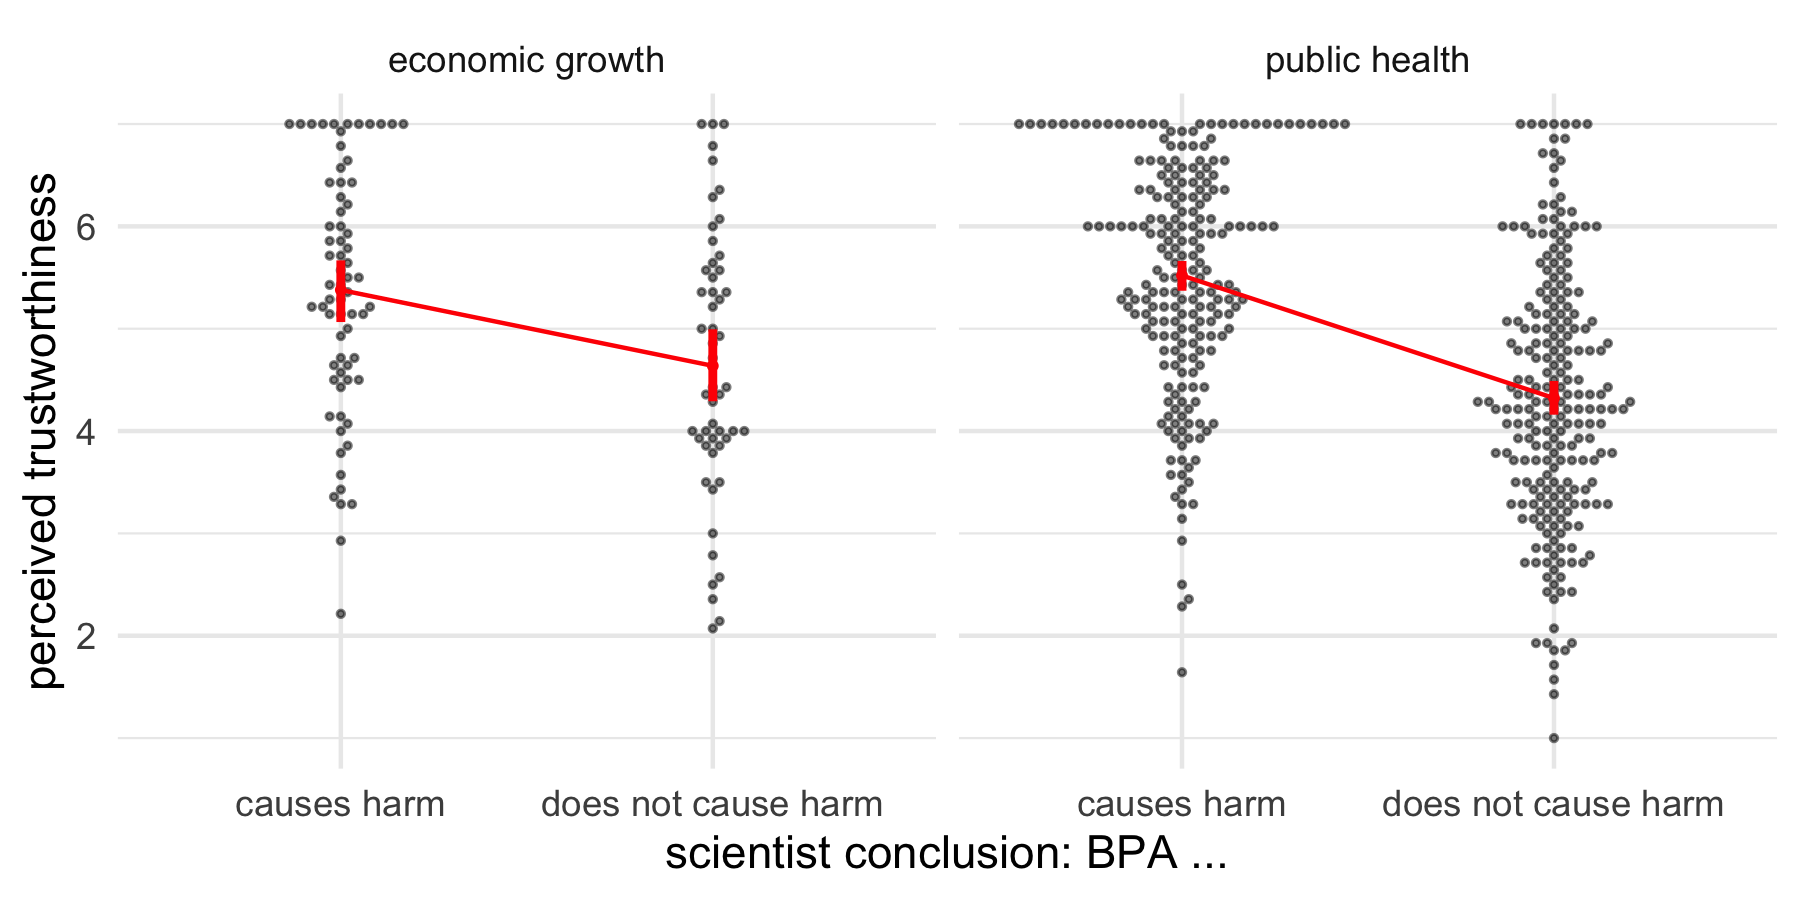
\includegraphics{fig4_conclusion_part.png}

}

\caption{\label{fig-conclusion-part}Data, group means, and 95\%
confidence intervals for H5-consumer, interaction of consumer risk
sensitivity and participant values. Panels correspond to participant
values.}

\end{figure}

\hypertarget{transparency-penalty}{%
\subsubsection{Transparency penalty}\label{transparency-penalty}}

To test whether the findings above about a hypothesized transparency
penalty may vary based on participants' values, we regressed
participants' METI ratings of the scientist onto the Disclosure
condition variable, Participants' Values variable, and the Disclosure by
Participants' Values interaction term. The full model was not
significant, adj. \(R^2\)\textless{} .001, \emph{F}(3, 840) = 1.19,
\emph{p} = .31 (Table~\ref{tbl-ec} model 2). As with the earlier
analysis, our results do not provide evidence for a transparency penalty
to the perceived trustworthiness of a scientist, either in general or
interacting with participants' own reported values, \(\beta\) = -0.23,
\emph{t}(840) = -1.07, \emph{p} = 0.286.

\hypertarget{tbl-ec}{}
\begin{table}
\caption{\label{tbl-ec}Regression analysis of H5-transparency, interaction between participant
values and transparency penalty }\tabularnewline

\centering
\resizebox{\linewidth}{!}{
\begin{tabular}{lccccccccc}
\toprule
\multicolumn{1}{c}{ } & \multicolumn{3}{c}{base} & \multicolumn{3}{c}{interaction} & \multicolumn{3}{c}{demographics} \\
\cmidrule(l{3pt}r{3pt}){2-4} \cmidrule(l{3pt}r{3pt}){5-7} \cmidrule(l{3pt}r{3pt}){8-10}
\textbf{Characteristic} & \textbf{Beta} & \textbf{95\% CI} & \textbf{p-value} & \textbf{Beta} & \textbf{95\% CI} & \textbf{p-value} & \textbf{Beta} & \textbf{95\% CI} & \textbf{p-value}\\
\midrule
(Intercept) & 5.1 & 4.9, 5.2 & <0.001 & 5.0 & 4.7, 5.3 & <0.001 & 4.9 & 4.3, 5.6 & <0.001\\
disclosure &  &  &  &  &  &  &  &  & \\
\hspace{1em}disclosure[TRUE] & -0.11 & -0.28, 0.06 & 0.2 & 0.04 & -0.32, 0.41 & 0.8 & 0.05 & -0.34, 0.43 & 0.8\\
part\_values &  &  &  &  &  &  &  &  & \\
\hspace{1em}part\_values[public health] &  &  &  & 0.07 & -0.26, 0.41 & 0.7 & 0.14 & -0.23, 0.51 & 0.5\\
\addlinespace
disclosure * part\_values &  &  &  &  &  &  &  &  & \\
\hspace{1em}disclosure[TRUE] * part\_values[public health] &  &  &  & -0.23 & -0.66, 0.19 & 0.3 & -0.29 & -0.74, 0.15 & 0.2\\
age &  &  &  &  &  &  & 0.00 & 0.00, 0.01 & 0.5\\
religious\_serv &  &  &  &  &  &  & 0.02 & -0.06, 0.09 & 0.7\\
political\_ideology &  &  &  &  &  &  & -0.02 & -0.08, 0.04 & 0.5\\
\addlinespace
education &  &  &  &  &  &  & -0.07 & -0.26, 0.11 & 0.4\\
\midrule
R² & 0.002 &  &  & 0.004 &  &  & 0.071 &  & \\
No. Obs. & 988 &  &  & 844 &  &  & 801 &  & \\
Adjusted R² & 0.001 &  &  & 0.001 &  &  & 0.009 &  & \\
Statistic & 1.60 &  &  & 1.19 &  &  & 1.15 &  & \\
\addlinespace
p-value & 0.2 &  &  & 0.3 &  &  & 0.2 &  & \\
\bottomrule
\multicolumn{10}{l}{\rule{0pt}{1em}\textsuperscript{1} CI = Confidence Interval}\\
\end{tabular}}
\end{table}

\hypertarget{shared-values-and-scientist-values}{%
\subsubsection{Shared values and scientist
values}\label{shared-values-and-scientist-values}}

Without adjustments, Shared Values appears to have a substantial
interaction with Participant Values: Shared Values appears to increase
perceived trustworthiness for participants who value public health,
while decreasing perceived trustworthiness for participants who value
economic growth (Figure~\ref{fig-shared-part}). However, as indicated by
our analysis for a potential shared values effect, the estimated effects
for both shared values and participant values are biased if the model is
not adjusted for scientist values. (Figure~\ref{fig-shared-dag} and
Table~\ref{tbl-shared} show how this bias occurs. Shared Values is a
collider between Participant Values and Scientist Values; hence, if a
model specification includes Participant Values and Shared values but
not Scientist Values, there is an open path between Participant Values
and METI, resulting in a biased estimate for Participant Values.)
Because Shared Values is the logical biconditional of Participant Values
and Scientist Values, and the Shared Values \(\times\) Participant
Values interaction term is their logical conjunction, including all four
variables (Participant, Scientist, and Shared Values, along with the
interaction term) in a regression model creates perfect collinearity.

\begin{figure}

{\centering 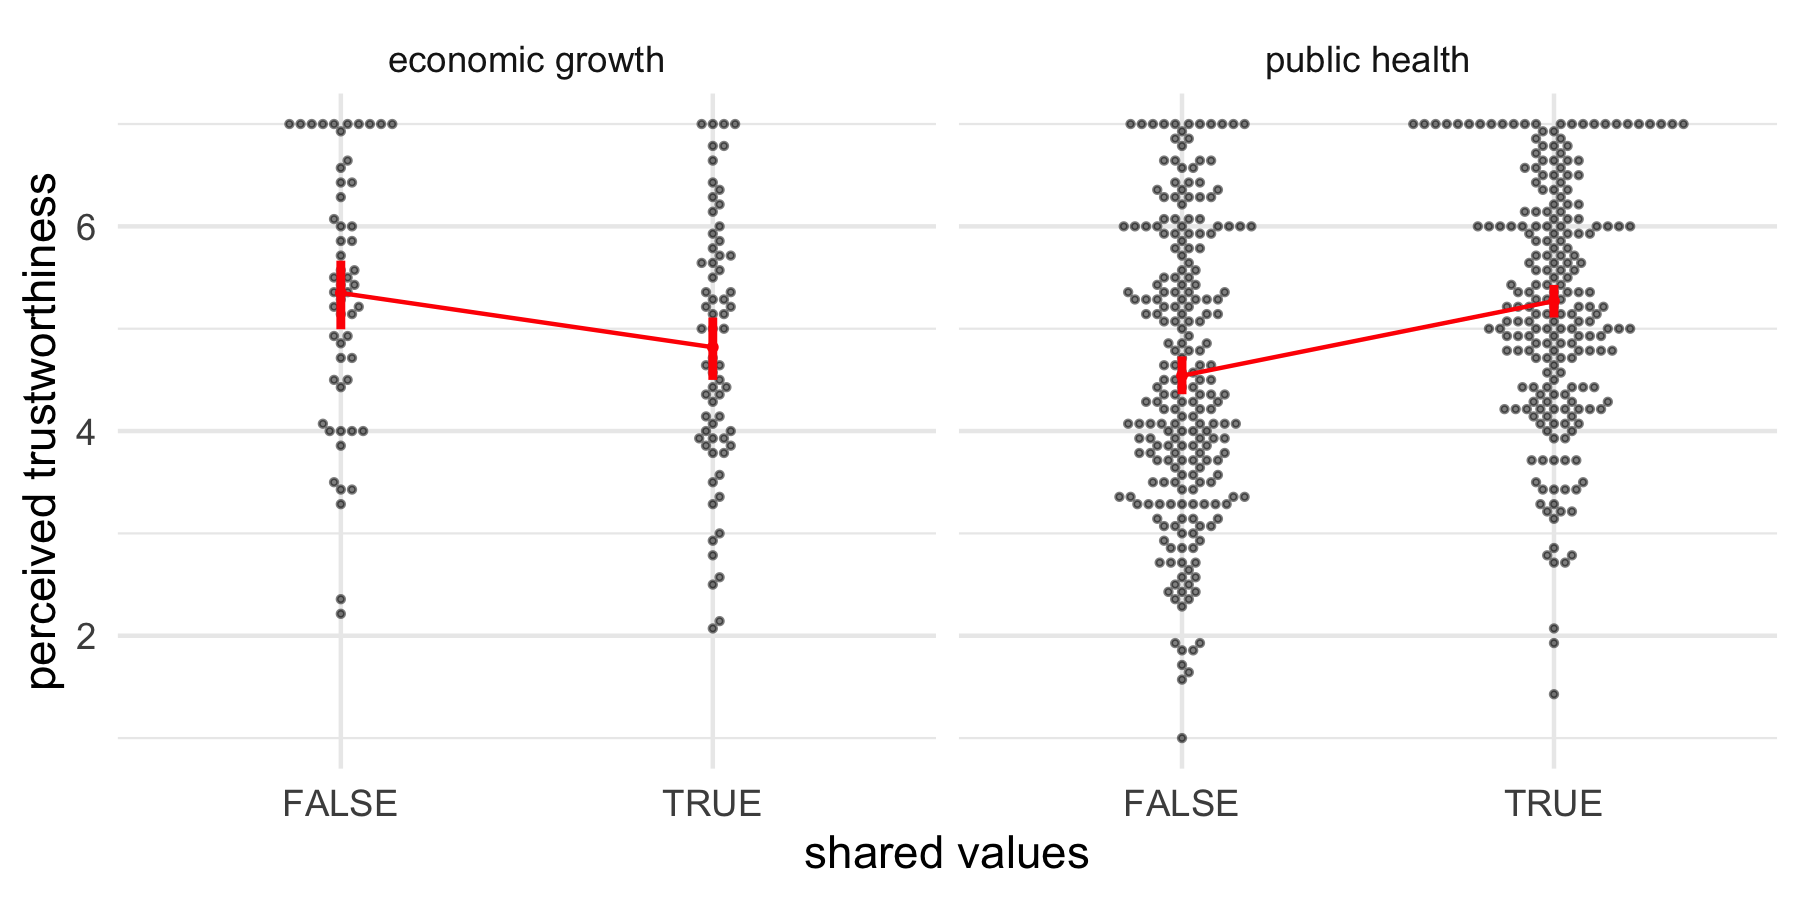
\includegraphics{fig5_shared_part.png}

}

\caption{\label{fig-shared-part}Data, group means, and 95\% confidence
intervals for H5-shared, interaction of shared values and participant
values. Panels correspond to participant values.}

\end{figure}

As we found above, rather than a shared values effect there appears to
be an effect of scientist values. Replotting the same data as
Figure~\ref{fig-shared-part} based on scientist values, rather than
shared values, suggests a more consistent effect across participant
values (Figure~\ref{fig-sci-part}). Therefore, we conducted an unplanned
post hoc analysis to test whether an effect of scientist values might
vary as a function of participants values. We regressed participants'
METI of the scientist in the stimulus onto the Scientist Values
variable, Participants' Values variable, and their interaction
(Table~\ref{tbl-sci-part}). This model was significant, adj. \(R^2\) =
0.065, \emph{F}(3, 563) = 14.15, \emph{p} \textless{} .001. The estimate
for the scientist values term was significant, \(\beta\) = 0.53,
\emph{t}(563) = 2.26, \emph{p} = 0.02, while the estimate for the
interaction term was not, \(\beta\) = 0.20, \emph{t}(563) = 0.75,
\emph{p} = 0.45. Estimates for both variables had large uncertainties,
with confidence intervals of about 1 (95\% confidence intervals,
scientist values: 0.07, 1.0; interaction term: -0.32, 0.72).

\begin{figure}

{\centering 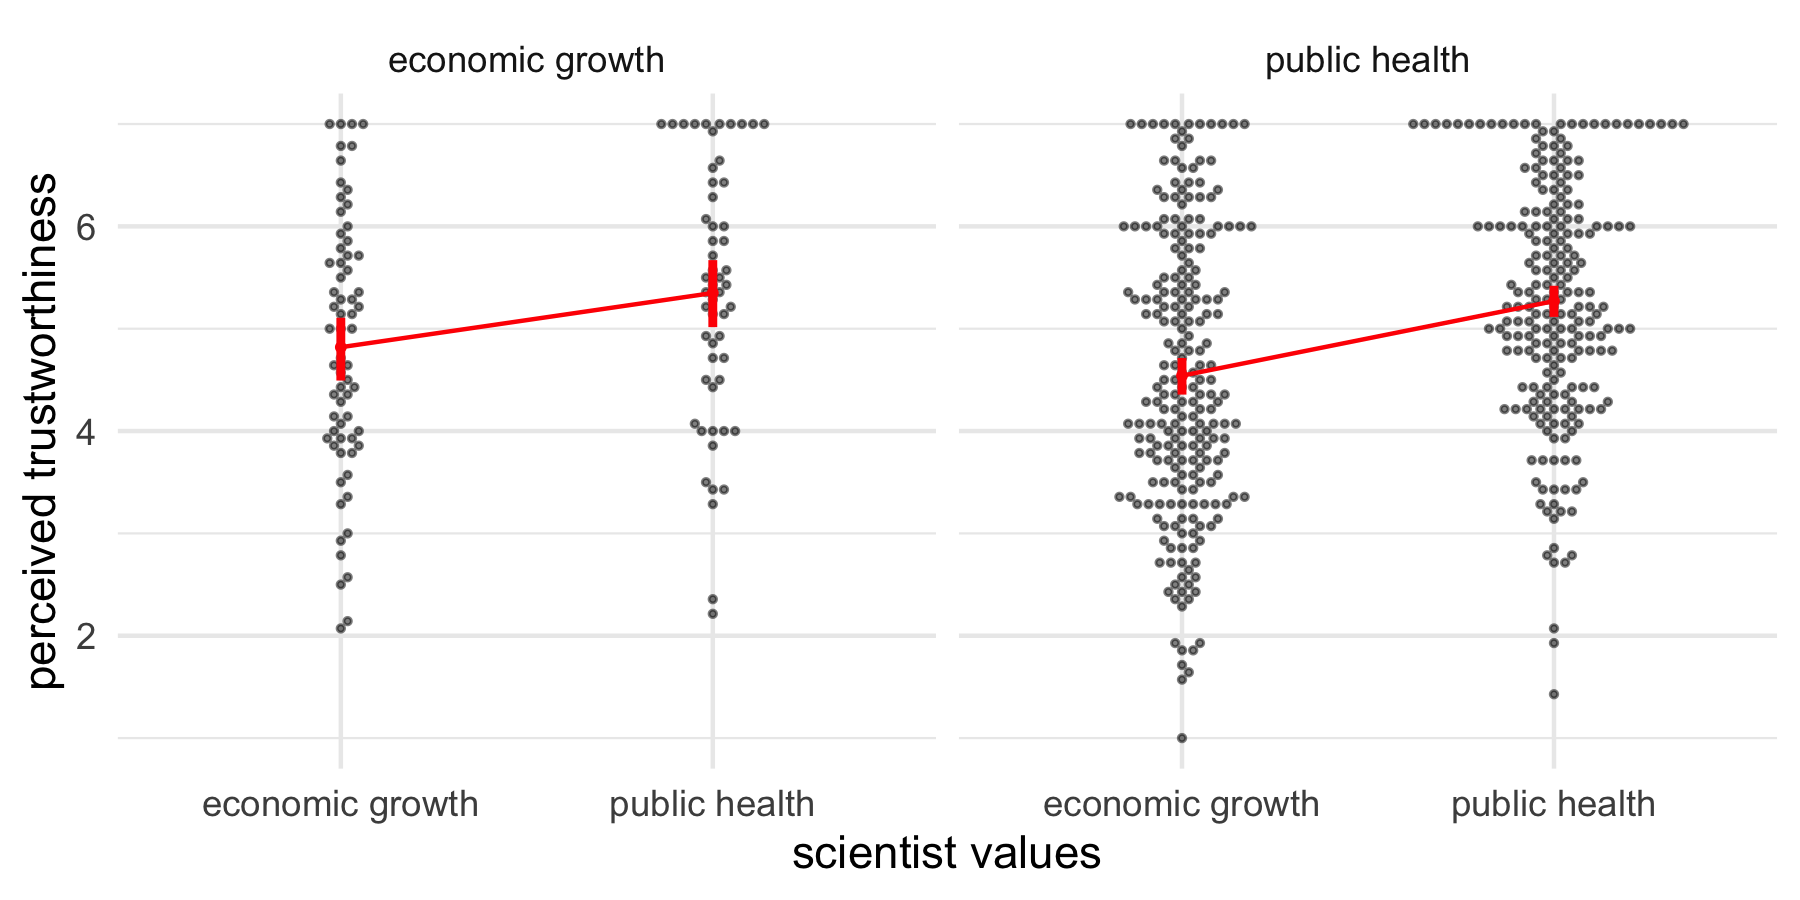
\includegraphics{fig6_sci_part.png}

}

\caption{\label{fig-sci-part}Data, group means, and 95\% confidence
intervals for a potential interaction of scientist values and
participant values. Panels correspond to participant values. This figure
is identical to Figure~\ref{fig-shared-part}, except the columns in the
economic growth panel have been switched.}

\end{figure}

\hypertarget{tbl-sci-part}{}
\begin{table}
\caption{\label{tbl-sci-part}Regression analysis of interaction between scientist values and
participant values }\tabularnewline

\centering
\resizebox{\linewidth}{!}{
\begin{tabular}{lcccccccccccc}
\toprule
\multicolumn{1}{c}{ } & \multicolumn{3}{c}{base} & \multicolumn{3}{c}{participant values} & \multicolumn{3}{c}{interaction} & \multicolumn{3}{c}{demographics} \\
\cmidrule(l{3pt}r{3pt}){2-4} \cmidrule(l{3pt}r{3pt}){5-7} \cmidrule(l{3pt}r{3pt}){8-10} \cmidrule(l{3pt}r{3pt}){11-13}
\textbf{Characteristic} & \textbf{Beta} & \textbf{95\% CI} & \textbf{p-value} & \textbf{Beta} & \textbf{95\% CI} & \textbf{p-value} & \textbf{Beta} & \textbf{95\% CI} & \textbf{p-value} & \textbf{Beta} & \textbf{95\% CI} & \textbf{p-value}\\
\midrule
(Intercept) & 4.6 & 4.5, 4.8 & <0.001 & 4.7 & 4.5, 5.0 & <0.001 & 4.8 & 4.5, 5.1 & <0.001 & 4.5 & 3.7, 5.4 & <0.001\\
sci\_values &  &  &  &  &  &  &  &  &  &  &  & \\
\hspace{1em}sci\_values[public health] & 0.65 & 0.45, 0.84 & <0.001 & 0.69 & 0.47, 0.90 & <0.001 & 0.53 & 0.07, 1.0 & 0.024 & 0.55 & 0.05, 1.1 & 0.031\\
part\_values &  &  &  &  &  &  &  &  &  &  &  & \\
\hspace{1em}part\_values[public health] &  &  &  & -0.19 & -0.44, 0.07 & 0.2 & -0.28 & -0.63, 0.08 & 0.12 & -0.24 & -0.65, 0.17 & 0.3\\
\addlinespace
sci\_values * part\_values &  &  &  &  &  &  &  &  &  &  &  & \\
\hspace{1em}sci\_values[public health] * part\_values[public health] &  &  &  &  &  &  & 0.20 & -0.32, 0.72 & 0.5 & 0.14 & -0.42, 0.71 & 0.6\\
age &  &  &  &  &  &  &  &  &  & 0.00 & -0.01, 0.01 & 0.7\\
religious\_serv &  &  &  &  &  &  &  &  &  & 0.01 & -0.08, 0.10 & 0.9\\
political\_ideology &  &  &  &  &  &  &  &  &  & -0.01 & -0.09, 0.06 & 0.8\\
\addlinespace
education &  &  &  &  &  &  &  &  &  & 0.05 & -0.18, 0.28 & 0.6\\
\midrule
R² & 0.060 &  &  & 0.069 &  &  & 0.070 &  &  & 0.143 &  & \\
No. Obs. & 660 &  &  & 567 &  &  & 567 &  &  & 538 &  & \\
Adjusted R² & 0.058 &  &  & 0.066 &  &  & 0.065 &  &  & 0.065 &  & \\
Statistic & 41.7 &  &  & 21.0 &  &  & 14.1 &  &  & 1.83 &  & \\
\addlinespace
p-value & <0.001 &  &  & <0.001 &  &  & <0.001 &  &  & 0.001 &  & \\
\bottomrule
\multicolumn{13}{l}{\rule{0pt}{1em}\textsuperscript{1} CI = Confidence Interval}\\
\end{tabular}}
\end{table}

\hypertarget{conclusion}{%
\section{Conclusion}\label{conclusion}}

Table~\ref{tbl-summary} summarizes the results of our replication
attempts. We were able to successfully replicate the correlation between
political ideology and valuing public health and consumer risk
sensitivity (a scientist who concludes BPA is harmful is perceived as
more trustworthy), and in addition found evidence of an interaction
between consumer risk sensitivity and whether the participant values
public health (participants who value public health have more extreme
reactions to the scientist's conclusion).

We did not find evidence for a transparency penalty or shared values
effect. And we found evidence of a scientist values effect (a scientist
who discloses valuing public health is perceived as more trustworthy),
which was not identified by Elliott et al. (2017).

\hypertarget{tbl-summary}{}
\begin{longtable}[]{@{}
  >{\raggedleft\arraybackslash}p{(\columnwidth - 4\tabcolsep) * \real{0.2471}}
  >{\raggedright\arraybackslash}p{(\columnwidth - 4\tabcolsep) * \real{0.5412}}
  >{\raggedright\arraybackslash}p{(\columnwidth - 4\tabcolsep) * \real{0.2118}}@{}}
\caption{\label{tbl-summary}Summary of replication results. 95\%
confidence intervals. \(^\star\)The shared values \(\times\) participant
values interaction specification had perfect multicollinearity and could
not be fit. \(^\dagger\)For these unplanned analyses, ``yes'' indicates
that we found evidence supporting the stated hypothesis, and ``no''
indicates that we did not find such evidence. \(^\ddagger\)Our analysis
method found no evidence of a shared values effect in the Elliott et al.
(2017) data.}\tabularnewline
\toprule()
\begin{minipage}[b]{\linewidth}\raggedleft
Hypothesis
\end{minipage} & \begin{minipage}[b]{\linewidth}\raggedright
\end{minipage} & \begin{minipage}[b]{\linewidth}\raggedright
Replicated? (CI)
\end{minipage} \\
\midrule()
\endfirsthead
\toprule()
\begin{minipage}[b]{\linewidth}\raggedleft
Hypothesis
\end{minipage} & \begin{minipage}[b]{\linewidth}\raggedright
\end{minipage} & \begin{minipage}[b]{\linewidth}\raggedright
Replicated? (CI)
\end{minipage} \\
\midrule()
\endhead
H1a & Liberals more likely to prioritize public health than
conservatives & yes \\
H1b & Majority of conservatives prioritize public health & no \\
H2 & Scientist who finds chemical is harmful perceived as more
trustworthy & yes (-1.1, -0.84) \\
H3 & Scientist who discloses values perceived as less trustworthy & no
(-0.28, 0.04) \\
H4 & Given scientist discloses values, scientist who shares values with
participant perceived as more trustworthy & no\(^\ddagger\) (-0.16,
0.36) \\
Unplanned & Given scientist discloses values, scientist who values
public health perceived as more trustworthy & yes\(^\dagger\) (0.37,
0.89) \\
H5-consumer & Conclusion (H2) \(\times\) participant values & yes
(-0.79, -0.04) \\
H5-transparenc & Disclosure (H3) \(\times\) participant values & no
(-0.66, 0.19) \\
H5-shared & Shared values (H4) \(\times\) participant values &
\(^\star\) \\
H5-sci. values & Scientist values \(\times\) participant values &
no\(^\dagger\) (-0.32, 0.72) \\
\bottomrule()
\end{longtable}

Elliott et al. (2017) claim evidence for a shared values effect by
comparing values disclosure vs.~no disclosure (that is, estimating a
transparency effect) in quasi-independent subsamples across a 2
\(\times\) 2 \(\times\) 2 design (participant values \(\times\)
scientist conclusion \(\times\) scientist values; Elliott et al. (2017)
fig.~1). This approach is difficult to interpret; their reasoning seems
to be that this estimate is statistically significant in 4/8 cells, and
in 3/4 of these cells (1 where respondent values economic growth) the
participant and scientist share values. But these analyses are
underpowered (for example, sample sizes are well below 100 for some of
the cells in which participants value economic growth) and the overall
approach cannot distinguish a shared values effect from other potential
effects (scientist values, participant values). Applying our regression
analysis approach to the data published by Elliott et al. (2017), the
estimate for shared values was not statistically significant, \(\beta\)
= 0.29, \emph{t}(335) = 1.75, \emph{p} = 0.08; while the estimate for
scientist values was statistically significant, \(\beta\) = 0.41,
\emph{t}(335) = 2.48, \emph{p} = 0.014. It seems likely that claims of a
shared values effect could have been an artifact of a less appropriate
analytic approach given the nature of the data.

The disagreement over a transparency penalty is more difficult to
explain. Using our approach and the data from Elliott et al. (2017), the
estimate for a values disclosure was statistically significant
(Table~\ref{tbl-bc} model 1). One possible explanation is that, over the
course of the COVID-19 pandemic, members of the general public have
become used to ``scientists'' (broadly including both bench researchers
and public health officials) making claims about the importance of
protecting public health. A values disclosure that might have been
regarded as violating the value-free ideal, pre-pandemic, might now be
seen as routine.

The scientist values effect --- a scientist who discloses valuing public
health is perceived as more trustworthy --- might be interpreted as
supporting some of the claims of the ``aims approach'' in philosophy of
science. This approach argues that scientific fields often have both
social or practical aims, along with epistemic aims such as the pursuit
of truth (Elliott and McKaughan 2014; Intemann 2015; Potochnik 2017;
Fernández Pinto and Hicks 2019; Hicks 2022). For example, the field of
public health might have the practical aim of promoting the health of
the public. Where certain values are seen as conflicting with these
aims, it is morally wrong for a scientist to promote those values.
Rather than violating the value-free ideal, a scientist who discloses
valuing public health might be seen as following the norms of the field
of public health.

All together, regarding the philosophical debates over values in
science, the evidence from this replication study suggests that the
effects of transparency on perceived trustworthiness might be
context-dependent. Transparency about the influence of might be
detrimental in some cases, beneficial in others, and neutral in still
others. Notably, both of the papers cited as objecting to transparency
(John 2017; Kovaka 2021) focus on climate change, while many of
Elliott's examples come from toxicology or environmental public health.
The critics might be right that transparency has undermined trust in the
climate context, while Elliott might be right that transparency can be
neutral or even beneficial in some public health contexts. Because
philosophers of science tend to work with a small number of rich case
studies, methods such as qualitative comparative analysis (QCA; Ragin
2013) would be worth exploring.

An obvious difference between climate and BPA is the public prominence
and political polarization of the two issues. For decades, the fossil
fuels industry has used a range of strategies to successfully attack the
perceived trustworthiness of climate scientists, especially in the minds
of conservative publics (Oreskes and Conway 2011; Supran and Oreskes
2017). While the chemical industry has also had a substantial influence
on the environmental safety regulatory system (Michaels 2008; Vogel
2013), controversies over BPA have received much less public attention.
A LexiNexis search indicates that uses of ``bisphenol'' in US newspapers
rose and then almost immediately fell around 2008, shortly after a US
consensus conference concluded that ``BPA at concentrations found in the
human body is associated with organizational changes'' in a number of
major physiological systems (vom Saal et al. 2007).

In more prominent and/or polarized cases than BPA, a number of other
psychological mechanisms might be activated. Motivated reasoning or
identity-protective cognition (Kahan et al. 2012) might cause members of
the general public to rate a scientist as more or less trustworthy
insofar as the scientist agrees with the respondent's ``side'' of the
debate, regardless of whether and which values are disclosed. That is,
the scientist conclusion might have a larger effect than scientist
values. Alternatively, respondents might use values disclosures to
identify which scientists are on ``their side,'' and so scientist values
would have a larger effect than scientist conclusion. Careful attention
to experimental design will be needed to separate these potential
multiway interactions between conclusions, disclosures, and public
prominence.

\hypertarget{limitations}{%
\subsection{Limitations}\label{limitations}}

As noted above, a major limitation of the current study is that the
sample substantially underrepresents political conservatives. Our
\emph{a priori} DAG analysis and empirical robustness checks do not
indicate any bias in our reported estimates due to this representation
problem. However, our estimates could still be biased if any of the
effects examined here have interactions with political ideology.

Another limitation is that our sample only considers US adults. It does
not include residents of any other country, and does not track where our
participants might live within the US. Public scientific controversies
often have different dynamics both across national borders and within
different regions of geographically large countries (Miles and Frewer
2003; Howe et al. 2015; Mildenberger et al. 2016; Mildenberger et al.
2017; Sturgis, Brunton-Smith, and Jackson 2021).

A third limitation is that the stimulus only considers a single
controversy, over the safety of the chemical bisphenol A (BPA). Public
attention to this controversy peaked around 2009. While it remains
unsettled in terms of both science and policy, it is much less socially
and politically salient than controversies over topics such as climate
change or vaccination. This limitation affects our ability to speculate
about the generalizability of our findings. That is, the effects we
reported may only apply narrowly to a subset of sociopolitically
controversial scientific topics that have not achieved the degree of
salience or persistence in sociopolitical discourse for as long as
topics like climate change or vaccinations.

\hypertarget{directions-for-future-work}{%
\subsection{Directions for future
work}\label{directions-for-future-work}}

The design from Elliott et al. (2017) assesses public perceptions of the
value-free ideal indirectly, by probing whether violations of this ideal
would lead to decreased perceived trustworthiness. But do members of the
general public accept the value-free ideal? Concurrently with this
replication study, we also asked participants directly for their views
on the value-free ideal and related issues and arguments from the
philosophy of science literature. A manuscript discussing this effort to
develop a ``values in science scale'' is currently under preparation.

We suggest three directions for future work in this area, two in the
experimental stimulus and one in the endpoint or outcome measured.

The stimulus developed by Elliott et al. (2017) involves a single
(fictional) scientist. But public scientific controversies often feature
conflicting claims made by contesting experts and counterexperts. For
example, as the Omicron wave of the COVID-19 pandemic waned in the US in
spring 2022, various physicians, public health experts, science
journalists, and government officials made conflicting claims about the
effective severity of Omicron, the relative effectiveness of masks in
highly vaccinated populations, and the need to ``return to normal''
(Adler-Bell 2022; Khullar 2022; Yong 2022). For members of the general
public, the question was not whether to trust the claims of a given
expert, but instead which experts to trust. Publics might perceive both
expert A and expert B to be highly trustworthy, but would need to make a
decision about who to trust if these experts are making conflicting
claims. It would be straightforward to modify the single-scientist
stimulus to cover this kind of ``dueling experts'' scenario. To modify
METI, participants might be asked which of the two experts they would
consider more competent, ethical, honest, etc. (Public scientific
controversies can include other prominent actors with no relevant
expertise, such as political journalists, elected officials, or social
media conspiracy theorists. Such individuals might nonetheless be
treated by publics as trusted sources for factual claims. Understanding
why many people might trust a figure like Alex Jones over someone like
Anthony Fauci would likely require prior work disentangling
trustworthiness, expertise, and institutional standing.)

Brown (2022) emphasized a distinction between individuals, groups, and
institutions, as both trustors and trustees, and argued that much of the
philosophical and empirical research on trust in science has focused on
either individual-individual trust (as in Elliott et al. (2017)) or
individual-group trust (as in the General Social Survey, which asks
individual respondents about their confidence in ``the scientific
community''). In future experiments, ``Dr.~Riley Spence'' could be
represented with an institutional affiliation, such as ``Dr.~Riley
Spence of the Environmental Protection Agency'' or ``Dr.~Riley Spence of
the American Petroleum Institute'' Or claims could be attributed
directly to institutions, such as ``Environmental Protection Agency
scientists'' or ``a report published by the American Petroleum
Institute.''

As noted above, ethicists make a distinction between trust and
trustworthiness. Instruments such as METI assess trustworthiness:
whether a speaker is perceived to have qualities that would make it
appropriate to trust them. Trust itself is closer to behavior than
attitudes, and would probably be better measured (in online survey
experiments and similar designs) by asking whether participants accept
claims made by speakers or support policy positions endorsed by
speakers. In addition, research on the climate controversy suggests that
acceptance of scientific claims might underpredict policy support. Since
2008, public opinion studies by the Yale Program on Climate Change
Communication have found that only about 50-60\% of the US public
understands that there's a scientific consensus on climate change, that
this understanding is politically polarized (conservatives are
substantially less likely to recognize the consensus), but also that
some climate policies enjoy majority support even among conservatives
(Leiserowitz et al. 2022). Putting these points together, future
research could ask participants whether they would support, for example,
increased regulation of BPA, either instead of or along with assessing
the perceived trustworthiness of the scientific expert.

\hypertarget{acknowledgments}{%
\section{Acknowledgments}\label{acknowledgments}}

For feedback on this project, thanks to Kevin Elliott and participants
at the Values in Science conference and Political Philosophy and Values
in Medicine, Science, and Technology 2022 conference.

\hypertarget{funding}{%
\section{Funding}\label{funding}}

Funding for this project was provided by the University of California,
Merced.

\hypertarget{references}{%
\section*{References}\label{references}}
\addcontentsline{toc}{section}{References}

\hypertarget{refs}{}
\begin{CSLReferences}{1}{0}
\leavevmode\vadjust pre{\hypertarget{ref-Adler-BellPandemicInterpreter2022}{}}%
Adler-Bell, Sam. 2022. {``The Pandemic Interpreter.''} Intelligencer.
February 24, 2022.
\url{https://nymag.com/intelligencer/2022/02/david-leonhardt-the-pandemic-interpreter.html}.

\leavevmode\vadjust pre{\hypertarget{ref-BaierTrustAntitrust1986}{}}%
Baier, Annette. 1986. {``Trust and Antitrust.''} \emph{Ethics} 96 (2):
231--60. \url{http://www.jstor.org/stable/2381376}.

\leavevmode\vadjust pre{\hypertarget{ref-BrownTrustExpertiseScientific2022}{}}%
Brown, Matthew. 2022. {``Trust, Expertise and Scientific Authority in
Democracy.''} Michigan State University, February 20.
\url{https://www.youtube.com/watch?v=y3XeP6e646g}.

\leavevmode\vadjust pre{\hypertarget{ref-CPSHistoricalTime2022}{}}%
{``CPS Historical Time Series Visualizations.''} 2022. United States
Census Bureau. March 12, 2022.
\url{https://web.archive.org/web/20220312234236/https://www.census.gov/library/visualizations/time-series/demo/cps-historical-time-series.html}.

\leavevmode\vadjust pre{\hypertarget{ref-CranorSocialBenefitsExpedited1995}{}}%
Cranor, Carl F. 1995. {``The Social Benefits of Expedited Risk
Assessments.''} \emph{Risk Analysis} 15 (3): 353--58.
\url{https://doi.org/10.1111/j.1539-6924.1995.tb00328.x}.

\leavevmode\vadjust pre{\hypertarget{ref-DouglasSciencePolicyValuefree2009}{}}%
Douglas, Heather E. 2009. \emph{Science, Policy, and the Value-Free
Ideal}. Pittsburgh, Pa: University of Pittsburgh Press.

\leavevmode\vadjust pre{\hypertarget{ref-ElliottTapestryValuesIntroduction2017}{}}%
Elliott, Kevin C. 2017. \emph{A Tapestry of Values: An Introduction to
Values in Science}. Oxford University Press.

\leavevmode\vadjust pre{\hypertarget{ref-ElliottValuesEnvironmentalResearch2017}{}}%
Elliott, Kevin C., Aaron M. McCright, Summer Allen, and Thomas Dietz.
2017. {``Values in Environmental Research: Citizens' Views of Scientists
Who Acknowledge Values.''} \emph{PLOS ONE} 12 (10): e0186049.
\url{https://doi.org/10.1371/journal.pone.0186049}.

\leavevmode\vadjust pre{\hypertarget{ref-ElliottNonepistemicValuesMultiple2014}{}}%
Elliott, Kevin C., and Daniel~J. McKaughan. 2014. {``Nonepistemic Values
and the Multiple Goals of Science.''} \emph{Philosophy of Science} 81
(1): 1--21. \url{https://doi.org/10.1086/674345}.

\leavevmode\vadjust pre{\hypertarget{ref-ElliottSciencePolicyTransparency2014}{}}%
Elliott, Kevin C., and David B. Resnik. 2014. {``Science, Policy, and
the Transparency of Values.''} \emph{Environmental Health Perspectives},
March. \url{https://doi.org/10.1289/ehp.1408107}.

\leavevmode\vadjust pre{\hypertarget{ref-FernandezPintoLegitimizingValuesRegulatory2019}{}}%
Fernández Pinto, Manuela, and Daniel J. Hicks. 2019. {``Legitimizing
Values in Regulatory Science.''} \emph{Environmental Health
Perspectives} 127 (3): 035001. \url{https://doi.org/10.1289/EHP3317}.

\leavevmode\vadjust pre{\hypertarget{ref-FunkAmericansPoliticsScience2015}{}}%
Funk, Cary, and Lee Rainie. 2015. {``Americans, Politics and Science
Issues.''} Pew Research Center.
\url{http://www.pewinternet.org/2015/07/01/americans-politics-and-science-issues/}.

\leavevmode\vadjust pre{\hypertarget{ref-GauchatPoliticizationSciencePublic2012}{}}%
Gauchat, Gordon. 2012. {``Politicization of Science in the Public Sphere
A Study of Public Trust in the United States, 1974 to 2010.''}
\emph{American Sociological Review} 77 (2): 167--87.
\url{https://doi.org/10.1177/0003122412438225}.

\leavevmode\vadjust pre{\hypertarget{ref-GoldenbergVaccineHesitancyPublic2021}{}}%
Goldenberg, Maya J. 2021. \emph{Vaccine Hesitancy: Public Trust,
Expertise, and the War on Science}. University of Pittsburgh Press.

\leavevmode\vadjust pre{\hypertarget{ref-GSSDataExplorer2022}{}}%
{``GSS Data Explorer.''} 2022. NORC at the University of Chicago. June
29, 2022.
\url{https://web.archive.org/web/20220629231111/https://gssdataexplorer.norc.org/variables/178/vshow}.

\leavevmode\vadjust pre{\hypertarget{ref-HendriksMeasuringLaypeopleTrust2015}{}}%
Hendriks, Friederike, Dorothe Kienhues, and Rainer Bromme. 2015.
{``Measuring Laypeople's Trust in Experts in a Digital Age: The Muenster
Epistemic Trustworthiness Inventory (METI).''} \emph{PLOS ONE} 10 (10):
e0139309. \url{https://doi.org/10.1371/journal.pone.0139309}.

\leavevmode\vadjust pre{\hypertarget{ref-HicksNewDirectionScience2014}{}}%
Hicks, Daniel J. 2014. {``A New Direction for Science and Values.''}
\emph{Synthese} 191 (14): 3271--95.
\url{https://doi.org/10.1007/s11229-014-0447-9}.

\leavevmode\vadjust pre{\hypertarget{ref-HicksWhenVirtuesAre2022}{}}%
---------. 2022. {``When Virtues are Vices: {`Anti-Science'} Epistemic
Values in Environmental Politics.''} \emph{Philosophy, Theory, and
Practice in Biology} 14 (0). \url{https://doi.org/10.3998/.2629}.

\leavevmode\vadjust pre{\hypertarget{ref-HoweGeographicVariationOpinions2015}{}}%
Howe, Peter D., Matto Mildenberger, Jennifer R. Marlon, and Anthony
Leiserowitz. 2015. {``Geographic Variation in Opinions on Climate Change
at State and Local Scales in the USA.''} \emph{Nature Climate Change} 5
(6): 596--603. \url{https://doi.org/10.1038/nclimate2583}.

\leavevmode\vadjust pre{\hypertarget{ref-IannoneGtEasilyCreate2022}{}}%
Iannone, Richard, Joe Cheng, and Barret Schloerke. 2022. {``Gt: Easily
Create Presentation-Ready Display Tables.''}
\url{https://CRAN.R-project.org/package=gt}.

\leavevmode\vadjust pre{\hypertarget{ref-IntemannDistinguishingLegitimateIllegitimate2015}{}}%
Intemann, Kristen. 2015. {``Distinguishing Between Legitimate and
Illegitimate Values in Climate Modeling.''} \emph{European Journal for
Philosophy of Science} 5 (2): 217--32.
\url{https://doi.org/10.1007/s13194-014-0105-6}.

\leavevmode\vadjust pre{\hypertarget{ref-JohnEpistemicTrustEthics2017}{}}%
John, Stephen. 2017. {``Epistemic Trust and the Ethics of Science
Communication: Against Transparency, Openness, Sincerity and Honesty.''}
\emph{Social Epistemology} 32 (2): 75--87.
\url{https://doi.org/10.1080/02691728.2017.1410864}.

\leavevmode\vadjust pre{\hypertarget{ref-KahanPolarizingImpactScience2012}{}}%
Kahan, Dan M, Ellen Peters, Maggie Wittlin, Paul Slovic, Lisa Larrimore
Ouellette, Donald Braman, and Gregory Mandel. 2012. {``The Polarizing
Impact of Science Literacy and Numeracy on Perceived Climate Change
Risks.''} \emph{Nature Climate Change} 2 (10): 732--35.
\url{https://doi.org/10.1038/nclimate1547}.

\leavevmode\vadjust pre{\hypertarget{ref-KennedyEvaluation2016Election2018}{}}%
Kennedy, Courtney, Mark Blumenthal, Scott Clement, Joshua D Clinton,
Claire Durand, Charles Franklin, Kyley McGeeney, et al. 2018. {``An
Evaluation of the 2016 Election Polls in the United States.''}
\emph{Public Opinion Quarterly} 82 (1): 1--33.
\url{https://doi.org/10.1093/poq/nfx047}.

\leavevmode\vadjust pre{\hypertarget{ref-KhullarWillCoronavirusPandemic2022}{}}%
Khullar, Dhruv. 2022. {``Will the Coronavirus Pandemic Ever End?''}
\emph{The New Yorker}, May 23, 2022.
\url{https://www.newyorker.com/news/daily-comment/will-the-coronavirus-pandemic-ever-end}.

\leavevmode\vadjust pre{\hypertarget{ref-KovakaClimateChangeDenial2021}{}}%
Kovaka, Karen. 2021. {``Climate Change Denial and Beliefs about
Science.''} \emph{Synthese} 198 (3): 2355--74.
\url{https://doi.org/10.1007/s11229-019-02210-z}.

\leavevmode\vadjust pre{\hypertarget{ref-LeePartyPolarizationTrust2021}{}}%
Lee, John J. 2021. {``Party Polarization and Trust in Science: What
about Democrats?''} \emph{Socius} 7 (January): 23780231211010101.
\url{https://doi.org/10.1177/23780231211010101}.

\leavevmode\vadjust pre{\hypertarget{ref-LeiserowitzPoliticsGlobalWarming2022}{}}%
Leiserowitz, Anthony, Edward Maibach, Seth Rosenthal, and John Kotcher.
2022. {``Politics \& Global Warming, April 2022.''} Yale Program on
Climate Change Communication.
\url{https://climatecommunication.yale.edu/publications/politics-global-warming-april-2022/}.

\leavevmode\vadjust pre{\hypertarget{ref-McKaughanBacktrackingEthicsFraming2013}{}}%
McKaughan, Daniel J., and Kevin C. Elliott. 2013. {``Backtracking and
the Ethics of Framing: Lessons from Voles and Vasopressin.''}
\emph{Accountability in Research} 20 (3): 206--26.
\url{https://doi.org/10.1080/08989621.2013.788384}.

\leavevmode\vadjust pre{\hypertarget{ref-MichaelsDoubtTheirProduct2008}{}}%
Michaels, David. 2008. \emph{Doubt is their product how industry's
assault on science threatens your health}. Oxford: Oxford Univ. Press.

\leavevmode\vadjust pre{\hypertarget{ref-MildenbergerDistributionClimateChange2016}{}}%
Mildenberger, Matto, Peter Howe, Erick Lachapelle, Leah Stokes, Jennifer
Marlon, and Timothy Gravelle. 2016. {``The Distribution of Climate
Change Public Opinion in Canada.''} \emph{PLOS ONE} 11 (8): e0159774.
\url{https://doi.org/10.1371/journal.pone.0159774}.

\leavevmode\vadjust pre{\hypertarget{ref-MildenbergerSpatialDistributionRepublican2017}{}}%
Mildenberger, Matto, Jennifer R. Marlon, Peter D. Howe, and Anthony
Leiserowitz. 2017. {``The Spatial Distribution of Republican and
Democratic Climate Opinions at State and Local Scales.''} \emph{Climatic
Change}, November, 1--10.
\url{https://doi.org/10.1007/s10584-017-2103-0}.

\leavevmode\vadjust pre{\hypertarget{ref-MilesPublicPerceptionScientific2003}{}}%
Miles, Susan, and Lynn J. Frewer. 2003. {``Public Perception of
Scientific Uncertainty in Relation to Food Hazards.''} \emph{Journal of
Risk Research} 6 (3): 267--83.
\url{https://doi.org/10.1080/1366987032000088883}.

\leavevmode\vadjust pre{\hypertarget{ref-OreskesMerchantsDoubtHow2011}{}}%
Oreskes, Naomi, and Erik M. Conway. 2011. \emph{Merchants of Doubt: How
a Handful of Scientists Obscured the Truth on Issues from Tobacco Smoke
to Global Warming}. New York, NY, USA: Bloomsbury.

\leavevmode\vadjust pre{\hypertarget{ref-PeerDataQualityPlatforms2021}{}}%
Peer, Eyal, David Rothschild, Andrew Gordon, Zak Evernden, and Ekaterina
Damer. 2021. {``Data Quality of Platforms and Panels for Online
Behavioral Research.''} \emph{Behavior Research Methods}, September.
\url{https://doi.org/10.3758/s13428-021-01694-3}.

\leavevmode\vadjust pre{\hypertarget{ref-PotochnikIdealizationAimsScience2017}{}}%
Potochnik, Angela. 2017. \emph{Idealization and the Aims of Science}.
Chicago and London: University of Chicago Press.

\leavevmode\vadjust pre{\hypertarget{ref-RCoreTeamLanguageEnvironmentStatistical2021}{}}%
R Core Team. 2021. {``R: A Language and Environment for Statistical
Computing.''} R Foundation for Statistical Computing.
\url{https://www.r-project.org/}.

\leavevmode\vadjust pre{\hypertarget{ref-RaginComparativeMethodMoving2013}{}}%
Ragin, Charles C. 2013. \emph{The comparative method: Moving beyond
qualitative and quantitative strategies}. Oakland, California:
University of California Press.

\leavevmode\vadjust pre{\hypertarget{ref-RepresentativeSamplesFAQ2022}{}}%
{``Representative Samples FAQ.''} 2022. Prolific. March 13, 2022.
\url{https://web.archive.org/web/20220313050153/https://researcher-help.prolific.co/hc/en-gb/articles/360019238413-Representative-samples-FAQ}.

\leavevmode\vadjust pre{\hypertarget{ref-vomSaalChapelHillBisphenol2007}{}}%
Saal, Frederick S. vom, Benson T. Akingbemi, Scott M. Belcher, Linda S.
Birnbaum, D. Andrew Crain, Marcus Eriksen, Francesca Farabollini, et al.
2007. {``Chapel Hill Bisphenol A Expert Panel Consensus Statement:
Integration of Mechanisms, Effects in Animals and Potential to Impact
Human Health at Current Levels of Exposure.''} \emph{Reproductive
Toxicology} 24 (2): 131--38.
\url{https://doi.org/10.1016/j.reprotox.2007.07.005}.

\leavevmode\vadjust pre{\hypertarget{ref-SjobergReproducibleSummaryTables2021}{}}%
Sjoberg, Daniel D., Karissa Whiting, Michael Curry, Jessica A. Lavery,
and Joseph Larmarange. 2021. {``Reproducible Summary Tables with the
Gtsummary Package.''} \emph{The R Journal} 13 (1): 570--80.
\url{https://journal.r-project.org/archive/2021/RJ-2021-053/index.html}.

\leavevmode\vadjust pre{\hypertarget{ref-SturgisTrustScienceSocial2021}{}}%
Sturgis, Patrick, Ian Brunton-Smith, and Jonathan Jackson. 2021.
{``Trust in Science, Social Consensus and Vaccine Confidence.''}
\emph{Nature Human Behaviour}, May, 1--7.
\url{https://doi.org/10.1038/s41562-021-01115-7}.

\leavevmode\vadjust pre{\hypertarget{ref-SupranAssessingExxonMobilClimate2017}{}}%
Supran, Geoffrey, and Naomi Oreskes. 2017. {``Assessing ExxonMobil's
Climate Change Communications (1977--2014).''} \emph{Environmental
Research Letters} 12 (8): 084019.
\url{https://doi.org/10.1088/1748-9326/aa815f}.

\leavevmode\vadjust pre{\hypertarget{ref-VogelItSafeBPA2013}{}}%
Vogel, Sarah A. 2013. \emph{Is It Safe?: BPA and the Struggle to Define
the Safety of Chemicals}. Oakland, California: University of California
Press.

\leavevmode\vadjust pre{\hypertarget{ref-WickhamWelcomeTidyverse2019}{}}%
Wickham, Hadley, Mara Averick, Jennifer Bryan, Winston Chang, Lucy
D'Agostino McGowan, Romain François, Garrett Grolemund, et al. 2019.
{``Welcome to the Tidyverse.''} \emph{Journal of Open Source Software} 4
(43): 1686. \url{https://doi.org/10.21105/joss.01686}.

\leavevmode\vadjust pre{\hypertarget{ref-YongHowDidThis2022}{}}%
Yong, Ed. 2022. {``How Did This Many Deaths Become Normal?''} The
Atlantic. March 8, 2022.
\url{https://www.theatlantic.com/health/archive/2022/03/covid-us-death-rate/626972/}.

\end{CSLReferences}



\end{document}
